%======================= ADVERSARIAL DETECTION IN DNN ===========================

\graphicspath{{img/adversarial/}}

\chapter{Adversarial Examples Detection in Deep Convolutional Image Classifiers}
\label{ch:adversarial}

%%% ABSTRACT
%
% Notwithstanding that, recent works have demonstrated that it is quite easy to create adversarial examples, i.e., images malevolently modified to cause deep neural networks to fail. Such images contain changes unnoticeable to the human eye but sufficient to mislead the network. This represents a serious threat for machine learning methods. In this paper, we investigate the robustness of the representations learned by the fooled neural network, analyzing the activations of its hidden layers.
% Specifically, we tested scoring approaches used for kNN classification, in order to distinguish between correctly classified authentic images and adversarial examples.
% These scores are obtained searching only between the very same images used for training the network.
% The results show that hidden layers activations can be used to reveal incorrect classifications caused by adversarial attacks.

As we can notice from the previous chapters, \acrfullpl{dcnn} are more and more pervading an increasing number of computer vision applications.
Noteworthy applications not considered in this thesis include image tagging~\cite{li2016socializing}, video captioning~\cite{baraldi2016hierarchical}, face verification~\cite{schroff2015facenet,parkhi2015deep}, super resolution~\cite{dong2016image}, just to name a few.
As the spread of \gls{dl}-based solution increases, also its adoption in sensible applications --- such as image forensics~\cite{tuama2016camera,bayar2016deep,zhang2016image,amerini2017localization}, spam/malware detection~\cite{dahl2013large}, and self-driving cars~\cite{cirecsan2012multi} --- increases accordingly.

Unfortunately, researchers shown that machine learning models, including deep learning methods, are highly vulnerable to adversarial examples~\cite{klarreich2016learning,goodfellow2014explaining,szegedy2013intriguing,papernot2016practical}.
An \emph{adversarial example} is a malicious input sample typically created applying a small but intentional perturbation such that the attacked model misclassifies it with high confidence~\cite{goodfellow2014explaining}.
In most of the cases, the difference between the original and perturbed image is imperceptible to a human observer.
Moreover, adversarial examples created for a specific neural network have been shown to be able to
fool different models with different architecture and/or trained on similar but different data~\cite{szegedy2013intriguing,papernot2016practical}.
These properties are known as cross-model and cross-dataset generalization of adversarial examples and imply that adversarial examples pose a security risk even under a threat model where the attacker does not have access to the target's model definition, model parameters, or training set~\cite{papernot2016practical,kurakin2016adversarial}.

It becomes crucial to understand how adversarial actions are perpetrated in order to consequently build up solutions to be robust against such attacks.
Most of the effort of the research community in defending from adversarial attacks had gone into increasing the model robustness to adversarial examples via enhanced training strategies, such as adversarial training~\cite{goodfellow2014explaining,papernot2016limitations} or defensive distillation~\cite{papernot2016distillation,grosse2016adversarial}.
%Fast adversarial generation methods~\cite{goodfellow2014explaining,papernot2016limitations} enable simple strategies such as adversarial training, that is the inclusion of adversarial examples generated on-the-fly in the training set.
%Other approaches~\cite{papernot2016distillation,szegedy2013intriguing} suggest to reduce or mask the classifier's decision surface and reduce the magnitude of the gradients towards adversarial points an attacker would exploit, or even completely mask the gradients using non-differentiable classifiers, such as kNNs.
However, studies have shown~\cite{papernot2016practical} that those techniques only increase the cost of adversarial example generation without completely solving the problem.
% - till now research tried to train models which are robust to this type of attacks, while no much work on detecting adversarial images
A parallel strategy recenly studied is to defend from adversarial attacks by distinguishing adversarial inputs from authentic inputs.
% - our contribution

\begin{figure}
\centering
\includegraphics[width=\linewidth]{figures/adv-det-overview}
\caption{Overview of our detection approach.
The input image is classified by the \gls{cnn}, but we consider the classification valid only if the kNN score of the predicted class based on a particular deep features is above a certain threshold.}
\label{fig:adv:overview}
\end{figure}

In this chapter, we present an approach to detect adversarial examples in deep neural networks based on the analysis of activations of the neurons in hidden layers --- also known as \emph{deep features} --- of the attacked neural network.
Being deep learning a subset of representation learning methods, we expect the learned representation to be more robust than the final classification to adversarial examples.
Moreover, adversarial images are generated in order to look similar to humans, and deep features have shown impressive results in visual similarity related tasks such as content-based image retrieval~\cite{sharif2014cnn,gordo2016deep}.
% Our main conjecture is the following,
% An authentic and its adversarial samples are almost identical at the input and produce very similar activations in the first layers of the network.
% Then, activations start diverging and produce completely different outputs.
% Our main conjecture is that we are able to tell adversarial samples from authentic ones looking at the intermediate activations of the network instead of its output.
Our investigation shows that, given an input image, searching for similar deep features among the images used for training allows us to predict the correctness of the classification produced by a \gls{cnn}.
In particular, we employ traditional kNN scoring approaches as a measure of the confidence of the classification given by the \gls{cnn}.
The score assigned by the kNN classifier to the class predicted by the \gls{cnn} is used as a confidence measure of the reliability of the predicted class.
The experiments show that we are able to filter out the majority of adversarial examples, while retaining most of the correctly classified authentic images.
The choice of the discriminative threshold is a trade-off between accepted false negatives (FN) and true positives (TP), where positive means non-adversarial.
%
% In this work, we present an approach to detect adversarial examples in deep neural networks, based on the similarity of intermediate network activations.
% Our main conjecture is the following.
% Since authentic and adversarial samples are very similar but activate the network in a very dissimilar way in the output layer, we should be able to discern the authentic samples from the adversarial ones looking at the network's intermediate activations.
% We show that kNN classifiers based on euclidean distances between intermediate layers' activations can be used to predict the correctness of the classification produced by a \gls{dnn}.
% In particular, the scores assigned by the kNN can be used as a measure of confidence on the predicted class.
% This allows to filter out many adversarial examples while retaining most of the correctly classified authentic images.

% For better understanding how an adversarial works, we'll start explaining briefly what is a Convolutional Network (because this model works well in visual tasks), then we'll describe what an adversarial example exploits to fool the classier and what happen in a ConvNet when this kind of image is given as input.

% This paper is and extended version of the work ``Detecting adversarial example attacks to deep neural networks'' by the same authors, submitted to the 2nd International Workshop on Multimedia Forensics and Security (MFSec 2017).
% In this version, we considered more hidden layers (\emph{pool5} and \emph{fc7}) and more kNN classification approaches (Weighted and Distance Weighted).
% We also added plots and a discussion about the cumulative distribution of scores (Figure \ref{fig:adv:score-densities}).

The chapter is structured as follows.
\ref{sec:adv:rel-work} reviews relevant work in the field of adversarial attacks and their analysis, and provides background knowledge about adversarial detection and generation algorithms.
In \ref{sec:adv:detection}, our approach to adversarial detection is presented, while in \ref{sec:adv:experiments} we describe the experimental settings we used to validate it.
Finally, \ref{sec:adv:conclusions} summarizes the main findings and presents some future research directions.

The research presented in this chapter was published in~\cite{carrara2017detecting,carrara2018adversarial}, and additional resources are available at \url{http://deepfeatures.org/adversarials/}.


\section{Adversarial Examples}
\label{sec:adv:rel-work}

One of the first works exploring adversarial examples for image classifiers implemented with convolutional neural network is the one of \citet{szegedy2013intriguing}.
The authors used a quasi-newtonian optimization method, namely L-BFGS, to find an image $\x_{adv}$ close to an original one $\x$ in terms of $L_2$ distance, yet differently classified.
They also have shown that the obtained adversarial images were also affecting different models trained on the same training set (\emph{cross-model generalization}) and also models trained with other yet similar training sets (\emph{cross-training set generalization}).
Cross-model and cross-training set generalization properties of adversarial examples are also confirmed in~\cite{tabacof2016exploring}, where the authors explored the pixel space around adversarial images moving in random directions applying different kinds of noise.
They show that adversarial images are not isolated, spurious points, but they occupy large regions of the pixel space that mislead models with similar classification boundaries.
While multipletheories has been proposed, the causes of the adversarial vulnerability of \gls{ml} models remain an open question.
Early explanations suggested that it is due to non-linearity of a deep neural networks and over-fitting~\cite{tabacof2016exploring}, while \citet{goodfellow2014explaining} argued that the primary cause of neural networks' vulnerability to adversarial perturbation is their linear nature.
In particular, the alignment between adversarial perturbations and weights in a high-dimensional dot product can cause high spourious activations even if small perturbations are given as input.

% \paragraph{Crafting algorithms}
To overcome to the high computational cost of the L-BFGS approach, \citet{goodfellow2014explaining} also proposed the \gls{fgsm} to efficiently find adversarial perturbations following the gradient of the loss function with respect to the image, which can be efficiently computed by back-propagation.
Many other methods derived from \gls{fgsm} have been proposed to efficiently craft adversarial images.
\citet{kurakin2016adversarial} proposed a basic iterative version of \gls{fgsm} in which multiple finer steps are performed to better explore the adversarial space.
\citet{dong2018boosting} proposed a version of iterative \gls{fgsm} equipped with momentum which won the NIPS Adversarial Attacks and Defences Challenge~\cite{kurakin2018adversarial} as best attack;
this resulted in adversarial images with an improved transferability among models.
% attacks we did not test but relevant to the field
Other attack strategies aim to find smaller perturbations using a higher computational cost.
\citet{nguyen2015deep} used evolutionary algorithms and gradient ascent optimization to produce fooling images which are unrecognizable to human eyes but are classified with high confidence by \glspl{cnn}.
%~\cite{papernot2016limitations} used forward derivatives to compute adversarial saliency maps that show which input feature have to be increased or decreased to produce the maximum perturbation of the last classification layer towards a chosen adversarial class.
% JSMA
In~\cite{papernot2016limitations}, a Jacobian-based saliency map is computed and used to greedily identify the best pixel to modify in order to steer the classification to the desired output.
% They also derived different metrics from adversarial saliency maps, such as \emph{hardness}, \emph{adversarial distance} and \emph{robustness}, to measure the ability of a model to cope with adversarial attacks.
% DeepFool
In~\cite{moosavi2016deepfool}, the classifier is locally linearized and a step toward the simplified classification boundary is taken, repeating the process until a true adversarial is reached.
% In~\cite{moosavi2016universal}, Moosavi et al. presented an algorithm to find image-agnostic (universal) adversarial perturbations for a given trained model, that are able fool the classifier with high probability when added to any input. % The authors also observed that universal adversarial perturbations show cross-model and cross-dataset generalization properties.
% Carlini Wagner
\citet{carlini2016towards} relied on a modified formulation of the adversarial optimization problem initially formalized by \citet{szegedy2013intriguing}.
They move the misclassification constraint in the objective function by adding a specifically designed loss term, and they change the variable of the optimization to ensure the obtained image is valid without enforcing the box constraint;
\gls{adam} is then employed to optimize and find better adversarial perturbations.
\citet{sabour2015adversarial} explored the manipulation of a particular internal representation of the network by means of adversarial inputs, showing that it is possible to move the representation closer to the one of a provided guide image.
% Features Adversarial  % to bypass our detector you have to change the evolution of all the features, not just one.
\citet{papernot2016practical} also shown that successfully attacks are possible even if the attacker does not have direct access to the model weights or architecture.
In fact, the authors successfully performed adversarial attacks to remotely hosted models, and \citet{kurakin2016adversarial} also showed that attacks in physical scenarios, such as feeding a model with a printout adversarial example through a digital camera, are possible and effective.

% - defenses
\paragraph{Defensive Strategies}
In the recent literature, a considerable amount of work has been dedicated to increasing the robustness of the attacked models to adversarial inputs.
In~\cite{szegedy2013intriguing}, the authors suggest to add a regularization term to the training loss based on the Lipschitz upper bound, that resembles a $L_2$ regularization, to limit the magnitude of the changes in the activations of a network caused by perturbations of the input.
\citet{gu2014towards} shown that denoising autoencoders can remove substantial amounts of the adversarial noise.
However, when stacking the autoencoders with the original neural network, the resulting network can again be attacked by new adversarial examples with even smaller distortion.
Thus, the authors proposed Deep Contractive Network, a model with an end-to-end training procedure that includes a smoothness penalty.
Fast crafting algorithms, such as \gls{fgsm}, enabled a defensive strategy called \emph{adversarial training}, in which adversarial examples are generated on the fly and added to the training set while training~\cite{goodfellow2014explaining,huang2015learning}.
While models that undergo adversarial training still suffer from the presence of adversarial inputs, the perturbation needed to reach them is usually higher, resulting in a higher detectability.
However, easily optimizable models, such as models with non-saturating linear activations, can be easily fooled due to their overly confident linear responses to points that not occur in the training data distribution~\cite{goodfellow2014explaining}.
This concept is also discussed in~\cite{papernot2016towards}, where the authors shows that there are tensions between model accuracy and resilience that has to be calibrated for each particular use case.
They also provide a detailed description of the threat model for a machine learning system according to adversarial goals and capabilities, and a categorization of attacks and defenses in this framework.
%\citet{papernot2016practical} argued that defense methods based on \emph{gradient masking}, that is denying the attacker a useful direction to find adversarial points, only increase the model robustness to small perturbations of the training manifold.
% distillation
In~\cite{papernot2015distillation,papernot2016distillation}, a two-phase training process known as \emph{distillation} is used to increase the robustness of a model to small adversarial perturbations by smoothing the model surface around training points and vanishing the gradient in the directions an attacker would exploit.
Still, attackers can find potential adversarial images using a non-distilled substitute model.
% Weak defences
Other defenses aim at removing the adversarial perturbation via image processing techniques, such as color depth reduction or median filtering of the image~\cite{xu2017feature,li2017adversarial}.
Despite performing well on specific attacks with very stringent threat models, they usually fail on white-box attacks~\cite{he2017adversarial}.

% - detection
Detection of adversarial examples is still an open problem~\cite{papernot2016limitations}.
In this direction, \citet{gong2017adversarial,metzen2017detecting} employed addidional sub-networks to detect whether the input is an adversarial example.
However, the proposed sub-network is still vulnerable to adversarial attacks, and a more complicate adversarial training procedure is needed to increase the robustness of the whole system.
\citet{feinman2017detecting,grosse2017statistical} relied on statistical tests for estimating the authenticity of a batch of samples by comparing against the disrtibution describing authentic inputs.
However, the main drawback of this method is the inability to perform a per-sample detection.

Despite many detection strategies have been proposed, yet results are far from satisfactory for all threat models~\cite{carlini2017adversarial}, and adversarial detection still pose a challenge.

\subsection{Adversarial Generation}
\label{sec:adv:algos}
In this subsection we provide a brief description of the two approaches %, namely \emph{box constrained L-BFGS} and \emph{Fast Gradient Sign},
we used in our work to generate adversarial images.
\paragraph{Box-constrained L-BFGS~\cite{tabacof2016exploring,szegedy2013intriguing}}
Given an input image $\x$ and a \gls{dcnn} classifier $\y = f(\x)$, an adversarial example is generated finding the smallest distortion $\eta$ such that $\x_\text{adv} = \x + \eta$ is misclassified by the target model, that is $f(\x+\eta) \neq \y$.
The adversarial perturbation $\eta$ is modeled as the solution of the following optimization problem:
\begin{equation} \label{eq:adv:box-optim}
\begin{split}
\underset{\eta}{\text{minimize}}&\qquad ||\eta|| + C \cdot \L(\y,\y^A) \\
\text{subject to} 				&\qquad L <= \x+\eta <= U, \\
                                &\qquad \y = f(\x+\eta) \,,
\end{split}
\end{equation}
where $L$ and $U$ are respectively lower and upper bound of pixel values, $f$ is the attacked classifier, $\L(\y,\y^A)$ is the cross-entropy loss computed between the output class probability distribution $\y$ and the target adversarial distribution $\y^A$ (which assigns probability 1 to the adversarial label and 0 to the remaining ones).
The parameter $C$ controls the trade-off between the magnitude of $\eta$ and its fooling power.
Lower values of $C$ lead to extremely small perturbations but may not be sufficient to fool the classifier.
An adversarial perturbation is found by solving \ref{eq:adv:box-optim} using the box-contrained L-BFGS optimization algorithm.
A first feasible value of $C$ is found with a coarse grid search and then tuned with a binary search.

\paragraph{\acrlong{fgsm}~\cite{goodfellow2014explaining}}
% This algorithm was first presented in~\cite{goodfellow2014explaining}.
In the \acrfull{fgsm}, the adversarial perturbation is proportional to the sign of the gradient back-propagated from the output to the input layer.
Mathematically speaking, let $\Theta$ the parameters of the model, $\x$ its input, $\y$ the targets (desired output) associated with $\x$, and $\L\( \x, \y, \Theta \)$ the loss function used to train the neural network.
The cost function can be linearized around the current value of $\Theta$, obtaining an optimal max-norm constrained perturbation
\begin{equation} \label{eq:adv:fgsm}
\eta = \varepsilon \cdot sign \( \nabla_{\x} \L\( \x, \y, \Theta \) \) \\.
\end{equation}
Note that the gradient can be computed easier using back-propagation.
The adversarial input is given by $\x_\text{adv} = \x + \eta$.

\paragraph{Iterative-\gls{fgsm}~\cite{kurakin2016adversarial}}
% follow gradient, make a step, clip, iterate
\citet{kurakin2016adversarial} improved the effectiveness of the \gls{fgsm} algorithm by proposing a basic iterative variation often called Iterative-\gls{fgsm} (I-\gls{fgsm}) or Basic Iterative Method (BIM).
Starting from the natural image $\x$, the iterative method applies multiple steps of \gls{fgsm} with a distortion $\varepsilon_i <= \varepsilon$.
The attack performs
\begin{equation} \label{eq:adv:i-fgsm}
\x_\text{adv}^0 = \x, \quad \x_{adv}^{i+1} = \text{clip}(\x_{adv}^{i} + \varepsilon_i \nabla\L(\x_{adv}^{i})) \,,
\end{equation}
where $\text{clip}(\cdot)$ ensures the image obtained at each step is in the valid range.
%Practically, an adversarial can be created by training an input image with these steps (notice that during the back-propagation pass the weights are freezed and not updated):
%\begin{itemize}
%\item Propagate the input $x$ forward to the output layer as in standard back-propagation.
%\item Calculate the error and back-propagate the gradient all the way to the input layer.
%\item Update the input with the perturbation such that we get the new input $x' = x + \eta$.
%\end{itemize}

\subsection{Attack Model}
\label{subsec:attack-model}

\citet{biggio2013evasion} categorized the kind of attack based on the knowledge of the attacker.
A \emph{zero-knowledge} adversary is the one producing adversarial examples for the classifier while being unaware of the defensive strategy deployed;
this scenario is usually over-optimistic since it considers a very limited adversary, but is the basic benchmark to test new detection algorithms.
Instead, a \emph{perfect-knowledge} adversary is aware of both the classifier and the detector and can access the parameters of both models;
this is the worst-case scenario in which the adversary has full control and on which many of the detection schemes are bypassed~\cite{carlini2017adversarial}.
A half-way scenario is the one with a \emph{limited-knowledge} adversary, that is aware of the particular defensive strategy being deployed, but does not have access to its parameters or training data.

In this work, we focus on the \emph{zero-knowledge} scenario and plan to test our approach in the other scenarios in future work.

% A preliminary version of the method we are proposing has been presented in~\cite{carrara2017detecting}.
%We extended that work taking into consideration different intermediate layers form which extract deep features to perform the detection.
%This led to the analysis of the robustness of the detection when varying different combinations of type of adversarial attacks and deep features, uncovering interesting aspects about the depth-wise transformation of the information represented in the network.

% \section{Background}
% \label{sec:adv:background}
% XXX reuse in background

%A \gls{dnn} has a multi-layered architecture where the activations of neurons of each layer can be seen as a representation of the \gls{dnn}'s raw input . The representation in each layer is obtained as a learned transformation of previous layer representation. The final layer encodes the information needed to solve a specific tasks on which the \gls{dnn} was trained, as for instance the set of classes that the \gls{dnn} is supposed to recognize.
%
% The main skill of \glspl{dnn} is the ability to take a raw input and transform it several times into representations each at a higher, slightly more abstract level, until the final output encodes the information needed to easily solve a given task.
%

%Deep learning methods are ``representation-learning methods with multiple levels of representation, obtained by composing simple but non-linear modules that each transform the representation at one level (starting with the raw input) into a representation at a higher, slightly more abstract level''~\cite{lecun2015deep}.

%Starting from 2012, deep learning has become state-of-the-art in image classification given the excellent results in ILSVRC challenges based on ImageNet ~\cite{krizhevsky2012imagenet,sermanet2013overfeat,Simonyan14c,szegedy2015going,he2016deep}.
%In the context of Content-Based Image Retrieval, deep learning architectures are used to generate high level features.
%The relevance of the internal representation learned by the neural network during training have been proved by many recent works~\cite{Bengio2013,lecun2015deep,amato2016yfcc100m,donahue2014decaf%,girshick2014rich}.
%In particular, the activation produced by an image within the intermediate layers of a deep convolutional neural network can be used as a high-level descriptor of the image visual content~\cite{sermanet2013overfeat,chandrasekhar2015practical,razavian2014cnn,amato2016yfcc100m, amato2016visual}.

%In this work, we employed the image representations extracted using OverFeat~\cite{sermanet2013overfeat}, a well-known and successful deep convolutional network architecture that have been studied for the analysis of adversarial attacks to convolutional neural networks~\cite{tabacof2016exploring}, and for which implementations of adversarial generation algorithms are publicly available (see \ref{sec:adv:experiments}).
%Specifically, we used the Fast OverFeat network pre-trained on ImageNet\footnote{Code and weights for OverFeat are publicly available at \url{https://github.com/sermanet/OverFeat}}, and we selected the activations of the \emph{pool5} layer as deep features for images.

\section{Detecting adversarial examples}
\label{sec:adv:detection}
%The intuition behind the technique we propose is the following.
%Even if adversarial images activate the last layers of the \gls{dnn} very differently than the original images, the corresponding activations of the lower layers, that is the deep features of an original and its adversarial image, still contains lower level informations common to both inputs.
%The internal representations of the \gls{dnn}, corresponding to the original and its adversarial image, diverge proceeding toward the output of the network. % not confirmed, hedging needed..

% Adversarial images are not isolated, spurious points of the pixel space near original images. Instead they are known to occupy large and compact regions of the input space near classification boundaries~\cite{tabacof2016exploring}.

We propose to detect adversarial examples analyzing the representation learned in the hidden layers (deep features) of the fooled convolutional neural networks.
%Being deep learning a subset of representation learning methods, we expect the learned representation to be more robust than the final classification to adversarial examples.

We claim that an intermediate representation used internally by the network is more robust than the final classification to adversarial examples.
This assumption is supported by two observations.
First, the vast majority of adversarial generation algorithms are not meant to fool the representation itself but only the final classification.
Second, adversarial images share most of the low-level visual appearance with the authentic images from which are generated, and intermediate features have shown to capture this similarity in many visual similarity related tasks~\cite{sharif2014cnn,gordo2016deep}.
%We decided to test kNN classifiers score assignments because they rely on those similarity among the representations.

To detect whether an image is tampered, we first classify it with the unsecured deep image classifier.
Then, the activations of an hidden layer are used as query to perform a kNN search on the training set of the model and to judge image similarity.
%In particular, we perform a kNN similarity search among the deep features obtained from the images used for training using as query a given image classified by the \gls{dnn}.
We then use the score assigned by a kNN classifier to the class predicted by the unsecured model as a measure of confidence of the classification.
Please note, we do not rely on the classification produced by the kNN, but we only use the score assigned to the class predicted by the deep neural network as a measure of confidence.

Formally, given a set of labeled images $\X = \{(\x_i, c_i)\}$ where $\x_i$ is an image and $c_i$ is its class label, a kNN classifier assigns labels to an unknown image $\q$ considering the ordered results of its $k$ nearest neighbors $NN(\q,k)=\{(\x_1,c_1) \ldots (\x_k,c_k)\}$ obtained performing a kNN search over $\X$ for a predefined distance function $d(\x, \y)$ between any two images.
We define the distance function as $d(\x,\y) = || \phi(\x) - \phi(\y) ||_2$, where $\phi(\x)$ is the internal activation extracted from the image $\x$ using the classifier, and $||\cdot||_2$ is the $L_2$ norm.
A score $s(\q,c)$ is assigned to every class $c$ found in the retrieved nearest neighbors of $\q$ as follows:
%Then, the class with the highest score is assigned to the unknown image $q$.
%The most common kNN classifier score function is:
\begin{equation} \label{eq:adv:knn-score}
s(\q,c) = \frac{\sum_{i=1}^{k} w_i \cdot \mathbbm{1}\{c_i = c\}}{\sum_{i=1}^{k} w_i} \\,
\end{equation}
where $\q$ is a query image, $c$ is the class for which we are computing the score, $c_i$ is the groundtruth class of the $i$-th result in $NN(\q,k)$, $w_i$ the weight assigned to the same $i$-th result, and $\mathbbm{1}\{c_i = c\}$ has value 1 if $c_i=c$, 0 otherwise.
In \ref{tab:adv:knn}, we report $w_i$ assignments for famous variants of kNN classifiers.

% \begin{table}
% \centering
% \begin{tabular}{|r l|}
% \hline
% Classifier & Weight \\\hline \hline
% kNN    &
% \parbox[c][10mm]{30mm}{$w_i = 1$} \\  \hline
% Weighted kNN  &
% \parbox[c][10mm]{30mm}{$w_i = \dfrac{1}{i}$} \\  \hline
% $d$-Weighted kNN &
% \parbox[c][10mm]{30mm}{$w_i = \dfrac{1}{d(q, x_i)^2}$}  \\
% \hline
% \end{tabular}
% \caption{Weighting functions for the various kNN Classifiers}
% \label{tab:adv:knn}
% \end{table}

\begin{table}
\newcolumntype{C}{>{\centering\arraybackslash}X}%
\centering
\begin{tabularx}{\linewidth}{CCC}
\toprule
             & \textsc{Weighted kNN} & \textsc{Distance-Weighted kNN} \\
\textsc{kNN} & \textsc{(W-kNN)} & \textsc{(DW-kNN)} \\
\midrule
$w_i = 1$ & $w_i = \dfrac{1}{i}$ & $w_i = \dfrac{1}{d(q, x_i)^2}$ \\ \bottomrule
\end{tabularx}
\caption{Weighting functions for the various kNN classifiers.}
\label{tab:adv:knn}
\end{table}

%Please note that for $k=1$ only $c_1$ has non-zero score. The class $c_q$ assigned by the kNN classifier to the unknown image $q$ is the class with the highest score:

%\begin{equation}\label{knn-classif}
%c_q = \argmax_c s(q,c)
%\end{equation}

%Please note that our strategy does not make use of the class predicted by the kNN classifier. Rather, to detect whether an input image is an adversarial example, we first use the \gls{dnn} to predict the class, then we use the kNN classifier to obtain a score for the class predicted by the \gls{dnn}.

Let $\x$ the input image and $c_{\x} = f(\x)$ the class predicted by the \gls{dcnn} with a forward computation.
The kNN classifier is used to compute the score $s(\x,c_{\x})$ of the class $c_{\x}$ predicted by the \gls{cnn}.
We decide that the classification is reliable --- i.e., it is not an adversarial example --- if the score $s(\x,c_{\x})$ is above a predefined threshold.
The score $s(\x, c_{\x})$ is basically a measure of the confidence of the classification given by the \gls{cnn}.
The intuition behind this choice is that while it is unlikely that a class correctly predicted by the \gls{cnn} has the highest kNN score among the scores of all the classes, it is implausible that a correct classification has a very low score.
%a very low score of the predicted class are implausible given that the class we are considered is the predicted one.
As anticipated, the choice of the score threshold controls trade-off between \acrfull{fpr} and \acrfull{tpr}, where the former is the rate of adversarial examples (negatives) not detected using the specific threshold (false), and the latter is the rate of correctly classified authentic images (positives) successfully identified (true).
Please note that we do not rely on additional models or data other than the fooled \gls{cnn} and its original training set for the extraction of deep features and for the detection task.
An overview of our complete pipeline is depicted in \ref{fig:adv:overview}.
%only rely on training data and we use the very same fooled neural network for extracting the deep features.

% As better detailed in next section, we used the OverFeat fast network~\cite{sermanet2013overfeat} pre-trained on ImageNet \gls{ilsvrc}'12 as \gls{cnn}. % considering \emph{pool5} as deep features.
% We performed tests using kNN classifiers defined on the \emph{pool5}, \emph{fc6}, and \emph{fc7} deep features.

%To decide whether an image being classified by OverFeat is an adversarial example or not, we used a kNN classifier choosing the \gls{ilsvrc}'12 training set as search set and the euclidean distance between deep features as the distance function $d(\cdot,\cdot)$.
%Our intuition is that the activations of intermediate layers of adversarial examples are distinguishable with high probability from the ones of the images belonging to the class the network is tricked to predict.
%Given an input image $x$, we compute the kNN score defined in \eqref{knn-score} of the class $c$ predicted by OverFeat, and we decide that the prediction is correct only if the score is above a certain threshold.

\section{Experimental Settings}
\label{sec:adv:experiments}
In this section, we describe the experimental setups used to evaluate the proposed adversarial detection approach.
Our method has been evaluated as a binary classification of the correctness of the prediction given by a \gls{cnn}, in which a positive outcome means that the prediction given by the \gls{cnn} is trustful, while a negative outcome indicates that the prediction given by the \gls{cnn} is spurious and have to be discarded.

We employed two datasets in the evaluation protocol: the \gls{ilsvrc}'12 subset of ImageNet~\cite{russakovsky2015imagenet} and the NIPS 2017 Adversarial Attacks and Defenses Kaggle Competitions~\cite{kurakin2018adversarial} DEV image set.
Both datasets share the same \gls{ilsvrc}'12 label space.
We selected these datasets for the experiments because of the big availability of classifiers pre-trained on \gls{ilsvrc}'12.
We search for similar images on the very same data that have been used for training the neural networks --- i.e., the \gls{ilsvrc}'12 training subset.
Thus, the kNN methods rely on the very same information the neural network have seen during training.

We performed experiments with two \gls{cnn} architectures.
First, we applied our approach to \emph{OverFeat-Fast} \gls{cnn}~\cite{sermanet2013overfeat} --- a well-known and successful deep convolutional network architecture that have been studied for the analysis of adversarial attacks to \glspl{cnn}~\cite{tabacof2016exploring} --- using a subset of the \gls{ilsvrc}'12 validation images to generate adversarial examples (\ref{subsec:adv:overfeat}).
Second, we aligned with the configuration proposed in the context of the NIPS 2017 Adversarial Defenses Kaggle Competition~\cite{kurakin2018adversarial}.
Therefore, we tested our method on the network used as baseline in the competition (\emph{InceptionV3}), and we used the DEV image set provided through Kaggle for the generation of adversarial examples (\ref{subsec:adv:inception}).

% Generated adversarials and other resources have been made public available\footnote{\url{http://deepfeatures.org/adversarials/}}.

\subsection{\emph{OverFeat-Fast} network}
\label{subsec:adv:overfeat}
In the experiments reported in this section, we selected the \emph{OverFeat-Fast} \gls{cnn}~\cite{sermanet2013overfeat} given that this network (trained network on \gls{ilsvrc}'12) was used in the papers in which both L-BFGS and \acrlong{fgsm} (see \ref{sec:adv:algos}) were presented.

As reported in \ref{sec:adv:detection}, our approach performs a kNN similarity search over the images that were used for training the attacked \gls{cnn} (the \gls{ilsvrc}'12 training set).
%We used the \gls{ilsvrc}'12 dataset~\cite{ILSVRC15} as a labeled set $X$ for the kNN classifiers and to generate adversarials images.
%It is composed by a training set of \textasciitilde 1.3M labeled images belonging to 1000 different classes (each having roughly between 900 and 1300 images), and a validation set containing 50 images for each of the 1000 classes, for a total of 50k labeled images.
%\paragraph{Image Selection}
For generating adversarial examples, we selected images from the \gls{ilsvrc}'12 validation set.
In particular, we selected two subsets of images based on the classification results.
The first set is composed by randomly selecting a correctly classified image for each of the 1,000 \gls{ilsvrc} classes, while the second set is composed by randomly selecting a wrongly classified image (for which the network has given a wrong prediction) for each of the same classes.
We could not select a wrongly classified image in the class coded ``n12057211'' (yellow lady's slipper, yellow lady-slipper, Cypripedium calceolus, Cypripedium parviflorum) because all the instances of this class in the validation set are correctly classified by OverFeat.
Thus, the two sets respectively count 1,000 and 999 images.
We named those subsets respectively \emph{Authentic} and \emph{Authentic Errors}, where `authentic' stands for non-adversarial images.

%\paragraph{Adversarial Generation}
For each image in the \emph{Authentic} subset, we generated two adversarial images using both box constrained L-BFGS\footnote{\url{https://github.com/tabacof/adversarial}} and \gls{fgsm}\footnote{\url{https://github.com/e-lab/torch-toolbox/tree/master/Adversarial}} algorithms.
For both methods, we used the default parameters in every generation, and we randomly selected the target class, that is the class we fool the network to predict.
We observed that L-BFGS algorithm failed to generate 8 adversarial images, in the sense that the class prediction of the generated adversarial image was the same of the original image.
Those failures in the generation process could be avoided by tuning the parameters of the algorithm for each input, but for sake of simplicity we discarded the failed adversarial examples, ending up with two sets of adversarial images respectively composed by 1,000 images generated by \gls{fgsm}, and 992 images obtained with L-BFGS.
The generated adversarial images are made publicly available\footnote{\url{http://deepfeatures.org/adversarials/}} to make easier to reproduce the experiments.

%\paragraph{Feature extraction}
We extracted the activations of the \emph{pool5}, \emph{fc6}, and \emph{fc7} intermediate layer of the pre-trained OverFeat fast network~\cite{sermanet2013overfeat} from the following sets of images: \emph{Authentic}, \emph{Authentic Errors}, \emph{L-BFGS Adversarial}, \emph{\gls{fgsm} Adversarial} and \emph{\gls{ilsvrc}'12 train set}.
Both fully connected layers \emph{fc6} and \emph{fc7} are composed by 4,096 floats, while activations of \emph{pool5} are composed by 1,024 6x6 feature maps.
Following~\cite{simonyan2014very}, we applied global average pooling (GAP) to the \emph{pool5} feature maps, which acts as a structural regularizer, obtaining an image representation of 1,024 floats.
For the kNN classifier, we used the features extracted from \gls{ilsvrc}'12 train set as labeled set $X$, and we defined the distance function $d(\q,\x)$ as the euclidean distance between the extracted features.
We chose $k=1,000$ to have a number of nearest neighbors of the same order of magnitude of the number of images per class in the labeled set. %because for each class we have roughly 1,000 images per class in the labeled set.
%For XXX we took the output before the ReLU activation function.
We tested also feature $L_2$-normalization and dimensionality reduction on extracted features using \gls{pca}+Whitening with 256 dimensionality.

%\paragraph{Adversarial detection and classification}
Given an input image $x$, we compute the kNN score $s(\x, c)$ for the class $c = f(\x)$ predicted by OverFeat, and we discard this classification if the score is below a certain threshold.
We computed the kNN score for each image in the \emph{\gls{fgsm} Adversarial}, \emph{L-BFGS Adversarial} and \emph{Authentic Errors} image sets, and for each set we measure the ability to detect an adversarial input as the performance of a binary classification problem (`trustful' / `spurious' classification).

% \subsection{Results}
% \label{subsec:adv:of-results}

In \ref{tab:adv:eer}, we report the detection accuracy of our proposed approach for different settings. % considering the {pool-5} hidden layer.
The accuracy of the binary `trustful' / `spurious' classification is evaluated in the \acrfull{eer} setting, that is when we choose a threshold yielding equal false positive and false negative rates.
% REV\#1: The features extracted have a rather high dimension. Are there potentially problems (e.g. curse of dimensionality) with KNN? Is that the reason why the PCA-based version performs better?
The best results were obtained processing the activations of the \emph{pool5} layer using \gls{pca} and Whitening, delivering an aggregated accuracy of roughly 85\% regardless of the adversarial generation method.
The three scoring approaches considered (see \ref{tab:adv:knn}) revealed similar performance with DW-kNN and W-kNN being more effective in detecting L-BFGS and \gls{fgsm}, respectively.

We found that adversarial examples generated with \gls{fgsm} are in general easier to detect using higher-level activations (\emph{fc6}, \emph{fc7}), while L-BFGS examples are significantly harder to filter out.
This is reasonable because the optimization problem solved by L-BFGS produces small adversarial perturbation that are usually more difficult to detect even at higher layers at the cost of a more time-consuming generation process.
While \emph{pool5} activations perform best when applying a considerable amount of preprocessing on them (PCA+Whitening), fully connected activations perform well when used as is.
We think a meaningful explanation for this behavior is given by the presence of dropout in the fully connected layers during the network training.
Dropout is known to reduce the co-adaptation of hidden units and help learning robust, independent representations~\cite{srivastava2014dropout}.
This may limit the benefits brought by dimensionality reduction schemes such as PCA.

\begin{table}
\renewcommand{\tabcolsep}{2.7pt}
\newcolumntype{R}{>{\raggedleft\arraybackslash}X}%
\newcolumntype{C}{>{\centering\sloppy\arraybackslash}X}%
\centering
\begin{tabularx}{\linewidth}{Xlcccccccccccc}
\toprule
                                                         &                & \multicolumn{4}{c}{\textsc{pool5}} & \multicolumn{4}{c}{\textsc{fc6}} & \multicolumn{4}{c}{\textsc{fc7}} \\
                                                                            \cmidrule(lr){3-6}                   \cmidrule(lr){7-10}                \cmidrule(lr){11-14}
\textsc{Proc.}                                           & \textsc{Score} & \footnotesize\sloppy\textbf{L-BFGS} & \footnotesize\textbf{FGSM} & \footnotesize\textbf{Aggr.} & \footnotesize\textbf{Err.}
                                                                          & \footnotesize\sloppy\textbf{L-BFGS} & \footnotesize\textbf{FGSM} & \footnotesize\textbf{Aggr.} & \footnotesize\textbf{Err.}
                                                                          & \footnotesize\sloppy\textbf{L-BFGS} & \footnotesize\textbf{FGSM} & \footnotesize\textbf{Aggr.} & \footnotesize\textbf{Err.} \\
\midrule
\multirow{3}{*}{None}                                    &    kNN & 70.7          & 69.9          & 70.3          & 58.1          & 76.4          & \textbf{88.8} & \textbf{82.2} & 65.8          & \textbf{77.0} & 87.8          & \textbf{82.1} & 67.0          \\
                                                         &  W-kNN & 71.2          & 70.8          & 71.0          & 59.6          & \textbf{77.0} & 86.9          & 81.7          & 68.0          & 73.2          & \textbf{88.8} & 80.3          & 69.7          \\
                                                         & DW-kNN & 71.0          & 69.9          & 70.4          & 58.6          & 76.3          & 88.6          & 82.0          & 65.2          & 76.7          & 87.8          & 81.9          & 66.7          \\ \midrule
\multirow{3}{*}{$L_2$-norm}                              &    kNN & 79.2          & 74.3          & 76.7          & 60.7          & 69.6          & 84.9          & 76.5          & 65.6          & 64.7          & 86.2          & 73.9          & 64.7          \\
                                                         &  W-kNN & 81.4          & 76.4          & 78.9          & 62.9          & 70.2          & 86.8          & 77.7          & 71.3          & 64.1          & 87.8          & 74.1          & 69.9          \\
                                                         & DW-kNN & 81.7          & 76.6          & 79.1          & 61.6          & 69.4          & 84.7          & 76.3          & 65.4          & 64.7          & 86.1          & 73.9          & 64.8          \\ \midrule
\multirow{3}{*}{\parbox[c][1.2cm]{1.2cm}{PCA +\\Whiten}} &    kNN & 86.4          & 83.4          & 84.9          & 62.9          & 67.5          & 84.8          & 75.2          & 66.2          & 63.4          & 86.3          & 73.1          & 64.6          \\
                                                         &  W-kNN & 85.9          & \textbf{83.8} & 84.8          & \textbf{65.0} & 68.6          & 86.6          & 76.6          & \textbf{72.0} & 62.7          & 88.0          & 73.2          & \textbf{70.5} \\
                                                         & DW-kNN & \textbf{86.5} & 83.5          & \textbf{85.0} & 63.6          & 67.9          & 84.4          & 75.3          & 66.0          & 63.6          & 85.9          & 73.1          & 64.8          \\
\bottomrule
\end{tabularx}
\caption{Detection accuracy in the \gls{eer} threshold setting for various activation layers, score functions, and features processing.
We report results for both type of adversarial (L-BFGS and FGSM) and the aggregated accuracy (Aggr.).
In the last column, we report the detection rate of erroneous classifications not due to adversarial examples.}
\label{tab:adv:eer}
\end{table}

\begin{figure}
\centering
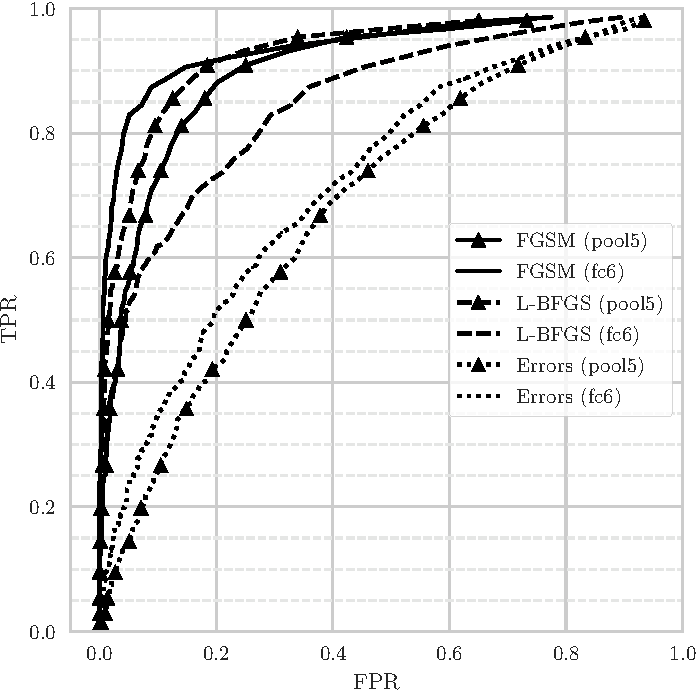
\includegraphics[width=.85\linewidth]{roc}
\caption{\gls{roc} curves of the binary classification (`prediction is right' or `prediction is wrong') for the various types of images.
The curves are obtained varying the discrimination threshold on the score assigned by the DW-kNN classifier to the class predicted by the CNN.
We only report the curves of the best performing configurations, that are \emph{fc6} with no processing, and \emph{pool5} with PCA and whitening.
Notice that when using \emph{pool5} we obtain a detection less sensible to a particular adversarial generation process.
}
\label{fig:adv:roc}
\end{figure}

In \ref{fig:adv:roc}, we report the \acrfull{roc} curves of the DW-kNN scoring approach on adversarial images and authentic errors.
The curves illustrate the performance of the proposed binary classifier when varying the threshold on the score $s(\x, f(\x))$.
%The results show that W-kNN is generally preferable when low FP rate are requested while DW-kNN is more effective when FP and TP are comparable.
As mentioned before, although \emph{fc6} performs better at detecting \gls{fgsm} adversarial examples, using \emph{pool5} activations result in a detector more robust in general.
However, we observed that higher kNN scores (which correspond to difficult L-BFGS adversarial to detect) usually reflects inter-class visual similarities that are independent from the adversarial nature of the input image (see \ref{tab:adv:bad-examples} for some examples).
The \gls{roc} curve for errors is the worst, indicating that our approach sometimes confuses authentic images that have been correctly and incorrectly classified.
As mentioned before, the detection of authentic images incorrectly classified (errors) would be a desirable property of our approach, but it is not our main goal.

\begin{figure}
\centering
%
\begin{subfigure}[t]{0.5\linewidth}
\centering
\textbf{pool5}\\
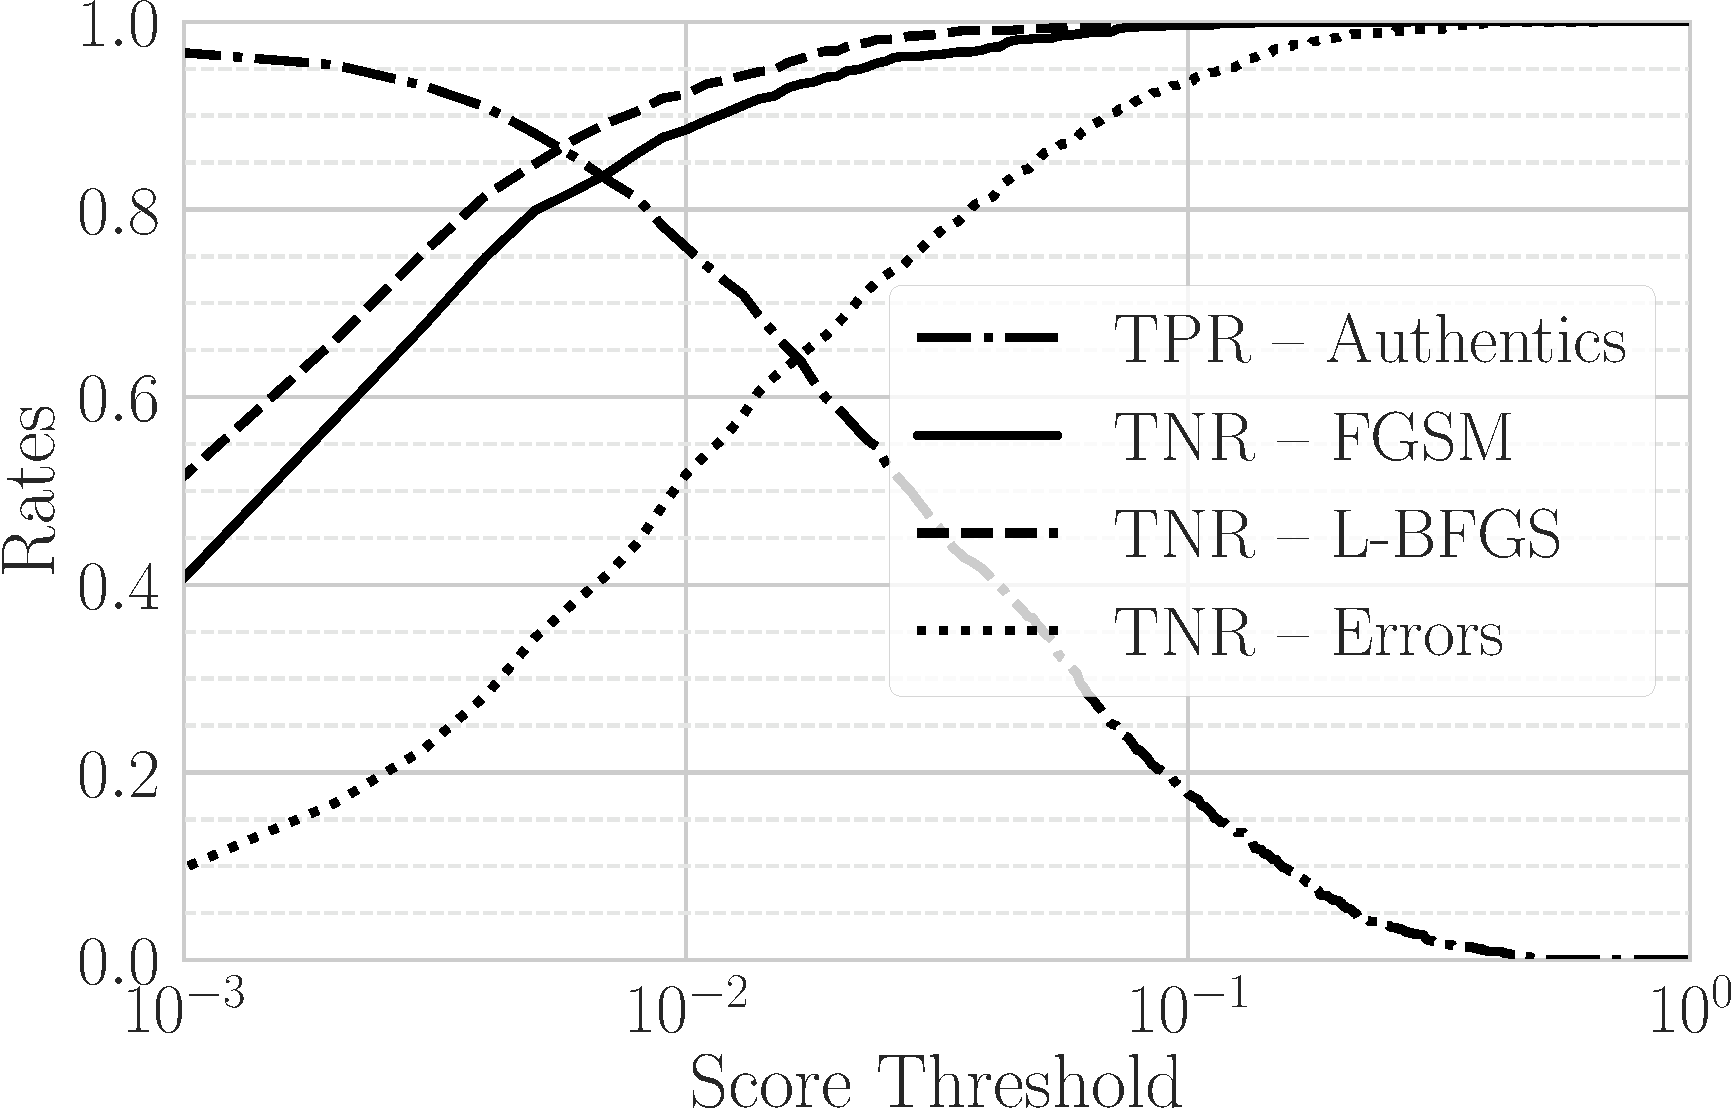
\includegraphics[width=\linewidth]{rates-pool5}%
\label{fig:adv:tpfn-dist-pool5}
\end{subfigure}%
%
\begin{subfigure}[t]{0.5\linewidth}
\centering
\textbf{fc6}\\
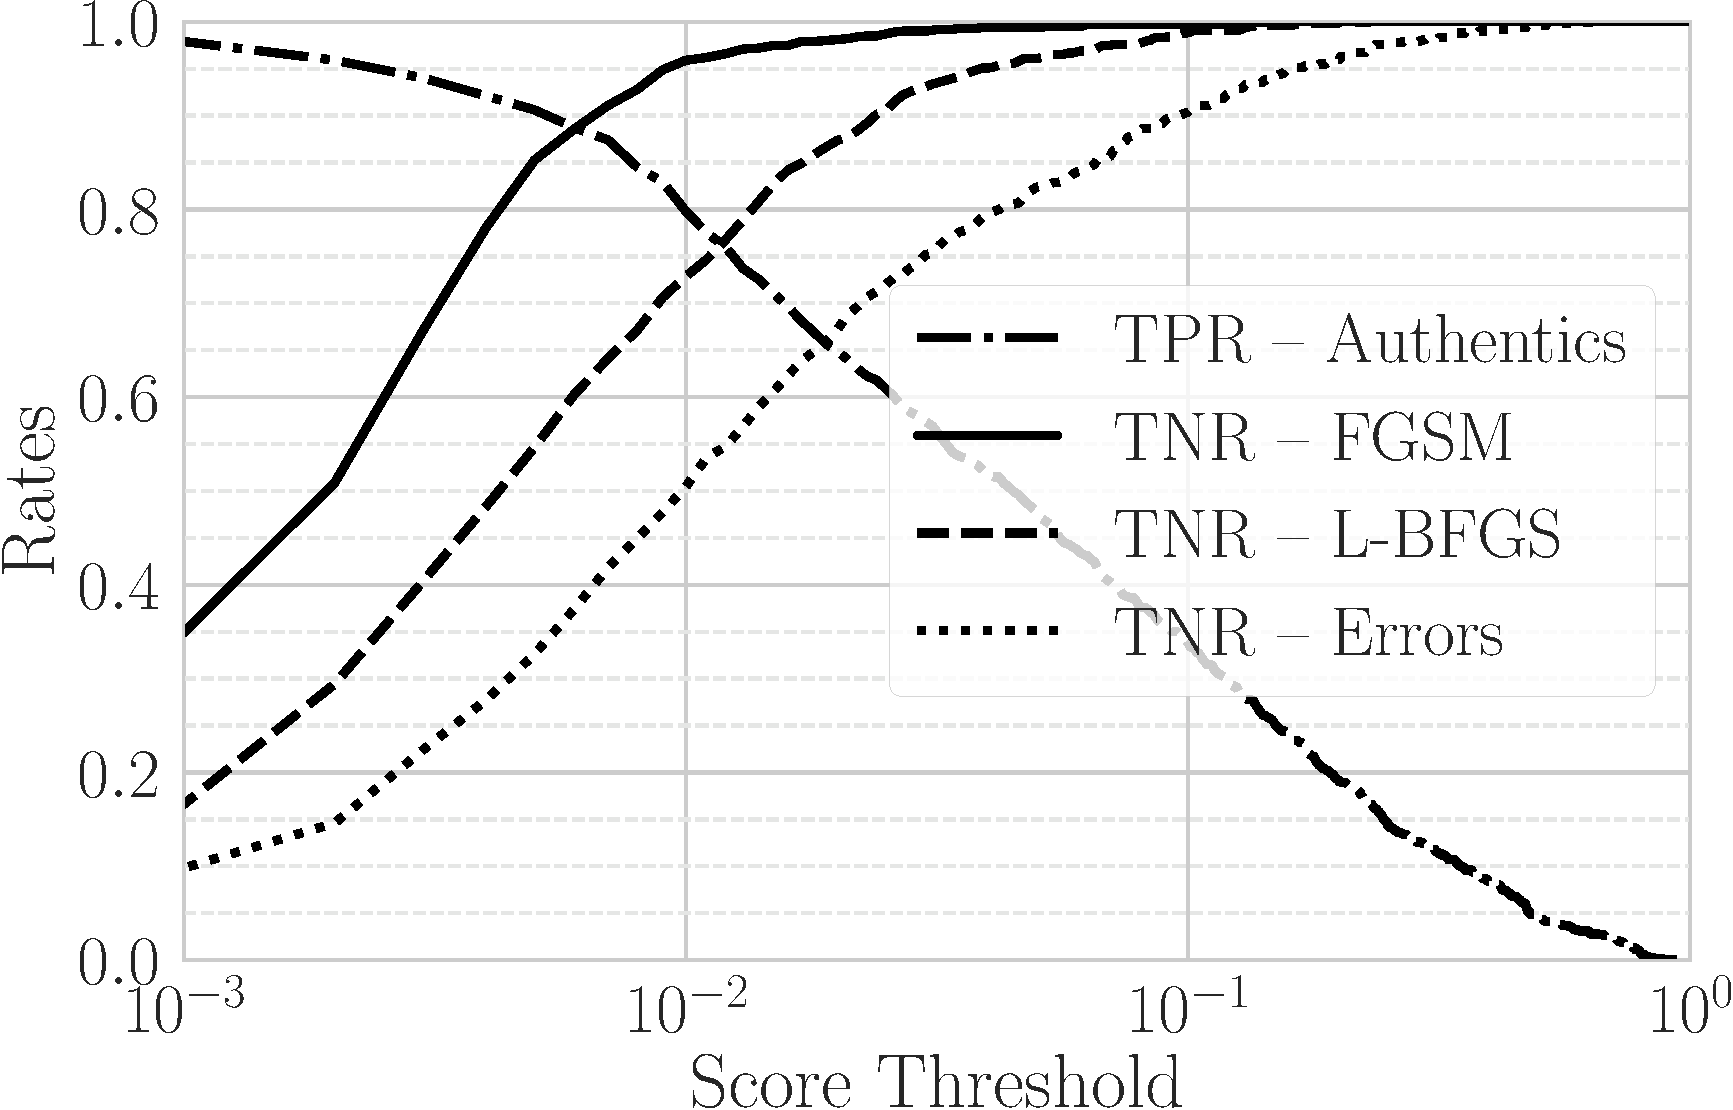
\includegraphics[width=\linewidth]{rates-fc6}%
\label{fig:adv:tpfn-dist-fc6}
\end{subfigure}%
\caption{True positive and true negative rates using as discrimination threshold between correctly and incorrectly classified images the score assigned by the DW-kNN classifier to the class predicted by the CNN.
The \emph{pool5} (on the left) and \emph{fc6} (on the right) layers have been used as features with PCA and Whitening processing.}
\label{fig:adv:tptn-distribs}
\end{figure}

Since we do not notice a prevalence of one of the three kNN weighting scheme tested, for the rest of the section, we will present results only for the DW-kNN scheme.
In \ref{fig:adv:tptn-distribs}, we report the true positive (for correctly classified authentic images) and true negative (for adversarial images and authentic errors) rates as a function of the discriminant threshold applied on the score $s(\x, f(\x))$.
Please note that for our method positive means non-adversarial.
We can easily note that using very low discrimination score values (about 0.002), it is possible to correctly filter out more than 50\% of the adversarial examples created by L-BFGS and more than 40\% of the ones created by \gls{fgsm}, while retaining more than 98\% of authentic images correctly classified.
As a positive side-effect, we also discard around 10\% of images the \gls{cnn} would misclassify.
The low threshold values reveal that while the DW-kNN score would not be effective in classifying the images, values below 0.003 are unlikely for authentic images.

The same results can be observer in the score densities reported in \ref{fig:adv:score-densities}, in which emerges a distinction between the score densities of adversarial images and the ones of authentic images.
Some simple statistics on those densities (such as the mean) could be computed online in the system hosting the model to isolate a particular source of adversarial examples, hence denying the access to the service to an attacker.

%In this paper, we focused on detecting individual adversarial examples. However, the results show that
%identifying as authentic more than 98\% of the images.
% \begin{table}[t]
% \small
% \centering
% \input{tab_clas}
% \caption{Accuracy of the classification using the kNN classification approach.}
% \label{tab:clas}
% \end{table}
% We also report the performance of the kNN classification approach, in which we predict the class of a given image taking the class having the maximum kNN score (see Equation \eqref{knn-classif}). Table \ref{tab:clas} shows the kNN classification accuracy for the different types of images we tested. While the kNN score helps in detecting adversarial examples, it is clear that it cannot be used to assign the correct class to adversarial examples, in particular for the images created using the FGS approach.

Finally in \ref{tab:adv:examples}, we report examples of successful detections and failures of our approach applied to the generated adversarial images. %, together with the nearest neighbor image in the kNN's labeled set and the score $s(x,f(x))$.
As anticipated, we observed that the most blatant failures (in which adversarial examples got higher scores) consist of attacks in which the target class share a strong visual similarity with the source original class -- e.g., an image of a Greater Swiss Mountain dog which is misclassified as a Bernese mountain dog.
In those difficult cases, intermediate representations of the target class are reasonable to lie around the ones of the original class in the feature space, and thus it is highly probable to erroneously obtain a confirmation of the classification of the \gls{cnn} by the kNN scoring approach.

\begin{table}
\centering
\newcommand{\imgside}{17mm}
\newcommand{\parside}{20mm}
\newcommand{\img}[1]{\parbox[c][\imgside]{\imgside}{\includegraphics[width=\imgside]{examples/#1}}}
%\newcommand{\pb}[1]{\parbox{\parside}{#1}}
\newcommand{\pb}[1]{#1}
\begin{subtable}{\linewidth}
\begin{tabularx}{\linewidth}{lcllcc}
\toprule
\textsc{Algorithm}&                            $\x_\text{adv}$ &                       \textsc{Actual} & \textsc{Predicted} & \textsc{1-NN} & $s$  \\
\midrule
L-BFGS   & \img{n02837789_ILSVRC2012_val_00004709_adversarial.png} & \pb{bikini, two-piece}                & pomegranate    & \parbox[c][\imgside]{\imgside}{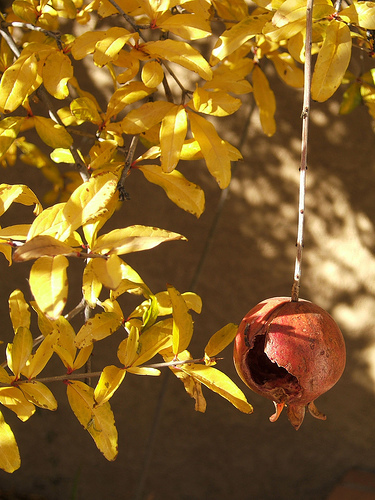
\includegraphics[width=\imgside,trim={0 1cm 0 3.5cm},clip]{examples/n07768694_863.JPEG}}   & 0.01 \\ \midrule
FGSM     & \img{n02892767_ILSVRC2012_val_00004599_adversarial.png} & \pb{brassiere, bra, bandeau}          & Chihuahua	    & \img{n02085620_10227.JPEG} & 0.01 \\ \midrule
FGSM     & \img{n04086273_ILSVRC2012_val_00011273_adversarial.png} & \pb{revolver, six-gun, six-shooter}   & mousetrap      & \img{n03794056_4688.JPEG}  & 0.00 \\ \midrule
L-BFGS   & \img{n02749479_ILSVRC2012_val_00039278_adversarial.png} & \pb{assault rifle, assault gun}       & Border terrier & \img{n02093754_3.JPEG}     & 0.00 \\
\bottomrule
\end{tabularx}
\caption{Examples of good detections of adversarial images with content that might be filtered. Low scores reflect a low confidence of image authenticity.\\[2ex]}
\label{tab:adv:good-examples}
\end{subtable}
\begin{subtable}{\linewidth}
\begin{tabularx}{\linewidth}{lclXcc}
\toprule
\textsc{Algorithm}&                            $\x_\text{adv}$ &                       \textsc{Actual} & \textsc{Predicted} & \textsc{1-NN} & $s$  \\
\midrule
FGSM     & \img{n03017168_ILSVRC2012_val_00041177_adversarial.png} & \pb{chime, bell, gong}      & barometer                                  &  \img{n02794156_12351.JPEG}  & 0.13 \\ \midrule
%L-BFGS   & \img{n02110806_ILSVRC2012_val_00025245_adversarial.png} & basenji                     & \pb{Arctic fox, white fox, Alopex lagopus} &  \img{n02120079_34796.JPEG}  & 0.13 \\ \midrule
L-BFGS   & \img{n02110806_ILSVRC2012_val_00025245_adversarial.png} & basenji                     & Arctic fox, white fox                      &  \img{n02120079_34796.JPEG}  & 0.13 \\ \midrule
FGSM     & \img{n02107574_ILSVRC2012_val_00033603_adversarial.png} & Greater Swiss Mountain dog  & Bernese mountain dog                       &  \img{n02107683_3087.JPEG}  & 0.11 \\ \midrule
FGSM     & \img{n03594945_ILSVRC2012_val_00041895_adversarial.png} & jeep, landrover             & pickup, pickup truck                       &  \img{n03930630_9160.JPEG}  & 0.11 \\
\bottomrule
\end{tabularx}
\caption{Examples of bad detections of adversarial images. Those are adversarial images for which our approach wrongly assigned a high score. However, this is mainly due to the visual similarity between the actual and fooled class.}
\label{tab:adv:bad-examples}
\end{subtable}

\caption{Examples of detections of adversarial images obtained by our best approach (\emph{pool5}+PCA+DW-kNN).
From left to right, columns respectively report: the adversarial generation algorithm, the generated adversarial image, its original class, the class predicted by the \gls{cnn}, the nearest neighbor image (in terms of $L_2$ distance between average-pooled \emph{pool5} activations) belonging to the predicted class, and the DW-kNN score $s$ for the predicted class.
A low score indicates that the adversarial is correctly detected (a) while a high score means that our approach is wrongly confident about the prediction of the CNN (b).
The results show that high scoring adversarial examples often share some common visual aspects and semantic with the predicted (adversarial) class, resulting in a more challenging detection.
}
\label{tab:adv:examples}
\end{table}

\begin{figure}
\centering%
%
\begin{subfigure}[t]{0.5\linewidth}%
\centering
\textbf{pool5}\\
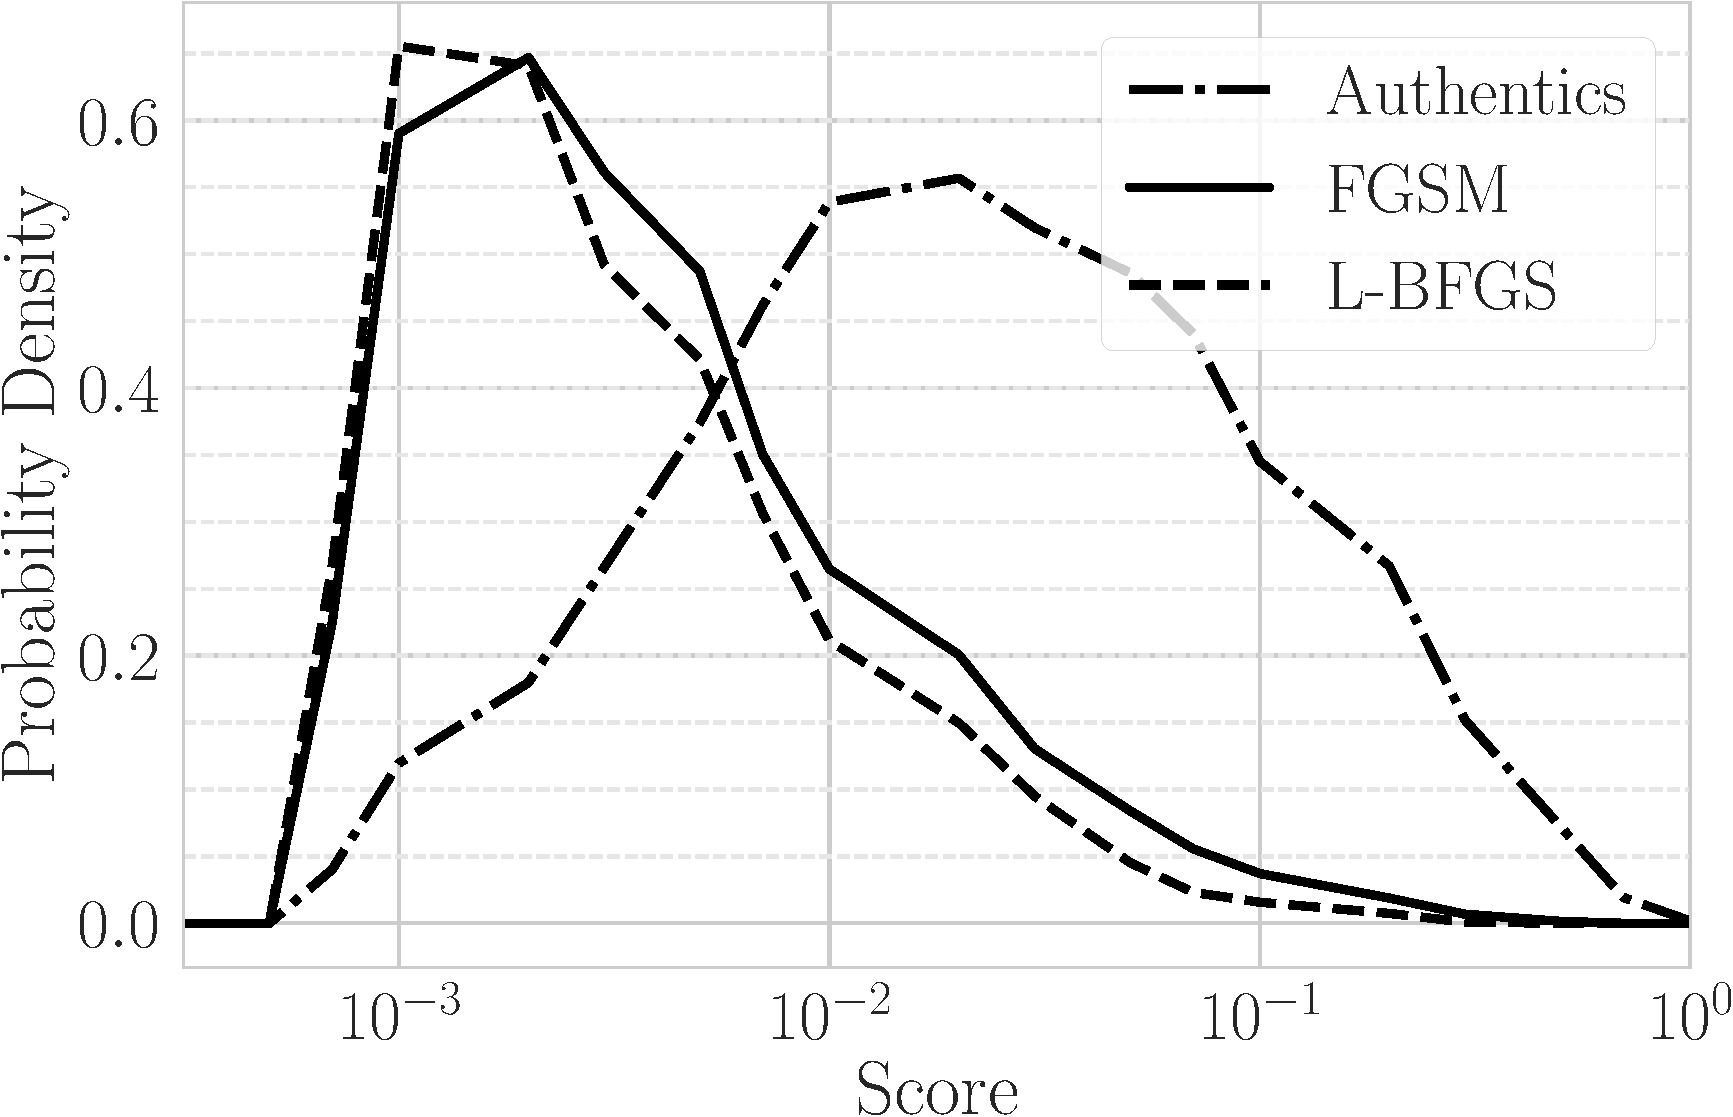
\includegraphics[width=\linewidth]{distrib-pool5}%
\label{fig:adv:score-density-pool5}%
\end{subfigure}%
%
\begin{subfigure}[t]{0.5\linewidth}%
\centering
\textbf{fc6}\\
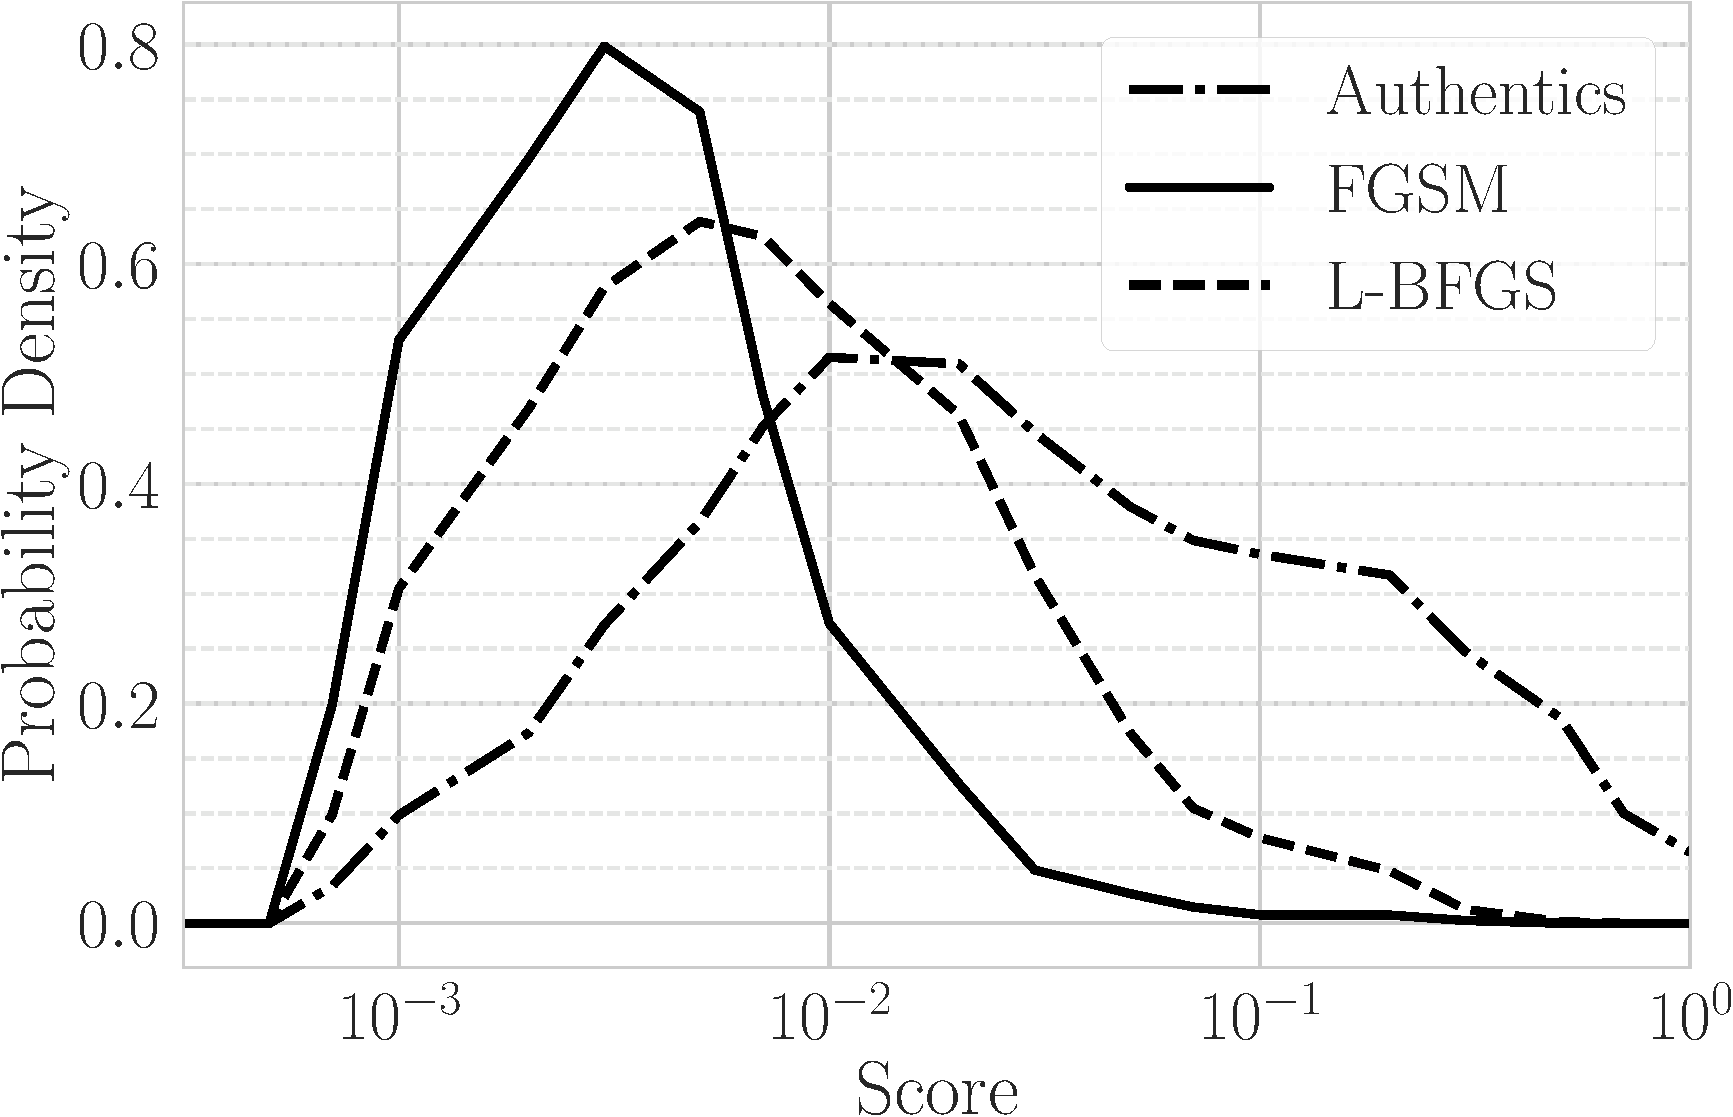
\includegraphics[width=\linewidth]{distrib-fc6}%
\label{fig:adv:score-density-fc6}%
\end{subfigure}%
%
\caption{Density of the DW-kNN scores for both adversarial and authentic images.
We report densities of scores using \emph{pool5} (on the left) and \emph{fc6} (on the right) as feature and PCA+Whitening as processing.}
\label{fig:adv:score-densities}
\end{figure}

\subsection{\emph{InceptionV3} Network on NIPS 2017 Adversarial Competition Dataset}
\label{subsec:adv:inception}

In the following experiments, we applied our detection algorithm to a more recent model, that is InceptionV3~\cite{szegedy2016rethinking}, which has been used as baseline classifier in the NIPS 2017 Adversarial Attacks and Defenses Kaggle Competitions~\cite{kurakin2018adversarial}.
Thus, instead of selecting random images from the \gls{ilsvrc}'12 validation set, we used the DEV images set released for the competition.
The DEV set is composed of 1,000 images that are not part of the ImageNet dataset, yet they have been manually labelled using the \gls{ilsvrc}'12 labels.

We followed the same methodology as in \ref{subsec:adv:overfeat}: we set apart from the DEV set the images that were incorrectly classified by InceptionV3; for the remaining images, we applied four different perturbation schemes (we generated the last two adversarial perturbations using the \emph{cleverhans} library~\cite{papernot2018cleverhans}):

%\SetLabelAlign{parright}{\parbox[t]{\labelwidth}{\bfseries \itshape \raggedleft#1}}
\begin{description}%[leftmargin=!,labelwidth=2.5cm, align=parright]
  \item[noop] the image is unchanged (authentic);
  \item[RandomNoise] the image is perturbed adding random gaussian noise in the interval $[-16, +16]$;
  \item[\gls{fgsm}] the image is perturbed with \gls{fgsm} (see \ref{sec:adv:algos}) with $\varepsilon = 16$ choosing a random target class;
  \item[I-\gls{fgsm}] the image is perturbed with 20 iterations of I-\gls{fgsm} algorithm with $\varepsilon = 1$; the target class is randomly chosen and kept fixed for all the iterations; the total perturbation is clipped to be in the interval $[-16, +16]$.
\end{description}

Since \textbf{RandomNoise} images are not meant to directly attack the classifier, we considered them authentic images. % together with the untouched images (\textbf{\emph{noop}}).
As in \ref{subsec:adv:overfeat}, we removed failed adversarial images produced by \textbf{\gls{fgsm}} or \textbf{I-\gls{fgsm}}, i.e., adversarial perturbed images for which the prediction of the network has not changed.
We also left out images produced by \textbf{RandomNoise} that are misclassified by the network, in order not to tamper the analysis of our adversarial detection approach with errors committed naturally by the classifier.
From this procedure, we obtained a test set comprising correctly classified authentic images and successfully generated adversarial images.

%For each image, we computed a score with our method for each proposed kNN scoring schemes (see \ref{sec:adv:detection}).
We performed a thorough exploration on the choice of the intermediate activation to be extracted from the InceptionV3 model.
We extracted convolutional features after each inception module, and we obtained compact representations applying global average pooling.
We also performed PCA dimensionality reduction to 256 components, since it had been proved beneficial for convolutional features in previous experiments (see \ref{subsec:adv:overfeat}).

% \subsubsection{Results}
% \label{subsec:adv:i3-results}

\begin{table}
\renewcommand{\tabcolsep}{3pt}
\newcolumntype{R}{>{\raggedleft\arraybackslash}X}%
\newcolumntype{C}{>{\centering\sloppy\arraybackslash}X}%
\begin{tabularx}{\linewidth}{Xcccccccccccc}
\toprule
                 & \multicolumn{4}{c}{\textsc{kNN}} & \multicolumn{4}{c}{\textsc{W-kNN}} & \multicolumn{4}{c}{\textsc{DW-kNN}} \\
                   \cmidrule(lr){2-5}                 \cmidrule(lr){6-9}                   \cmidrule(lr){10-13}
\textsc{Layer}   &  \multicolumn{1}{c}{\footnotesize\textbf{FGSM}} &  \multicolumn{1}{c}{\sloppy\footnotesize\textbf{I-FGSM}} &  \multicolumn{1}{c}{\footnotesize\textbf{Aggr.}} &  \multicolumn{1}{c}{\footnotesize\textbf{Err.}}
                 &  \multicolumn{1}{c}{\footnotesize\textbf{FGSM}} &  \multicolumn{1}{c}{\sloppy\footnotesize\textbf{I-FGSM}} &  \multicolumn{1}{c}{\footnotesize\textbf{Aggr.}} &  \multicolumn{1}{c}{\footnotesize\textbf{Err.}}
                 &  \multicolumn{1}{c}{\footnotesize\textbf{FGSM}} &  \multicolumn{1}{c}{\sloppy\footnotesize\textbf{I-FGSM}} &  \multicolumn{1}{c}{\footnotesize\textbf{Aggr.}} &  \multicolumn{1}{c}{\footnotesize\textbf{Err.}} \\
\midrule
maxpool\_5a\_3x3 &          50.1 &          51.9 &          51.1 &          31.1 &          58.2 &          60.8 &          59.7 &          45.6 &          58.3 &          60.9 &          59.8 &          45.7 \\
mixed\_5b        &          53.0 &          54.4 &          53.8 &          35.4 &          59.5 &          63.0 &          61.5 &          49.1 &          59.5 &          63.0 &          61.5 &          49.1 \\
mixed\_5c        &          56.6 &          58.4 &          57.6 &          41.2 &          62.2 &          66.9 &          64.9 &          54.6 &          62.2 &          66.9 &          64.9 &          54.5 \\
mixed\_5d        &          57.6 &          59.8 &          58.9 &          43.2 &          63.8 &          68.7 &          66.6 &          57.5 &          63.8 &          68.8 &          66.6 &          57.8 \\
mixed\_6a        &          62.6 &          65.7 &          64.4 &          51.5 &          68.7 &          74.4 &          72.0 &          61.7 &          68.8 &          74.4 &          72.0 &          62.7 \\
mixed\_6b        &          62.3 &          72.7 &          68.2 &          52.8 &          67.8 &          79.9 &          74.7 &          63.1 &          68.0 &          80.0 &          74.8 &          64.0 \\
mixed\_6c        &          70.7 &          80.6 &          76.3 &          60.5 &          71.0 &          82.5 &          77.6 &          68.2 &          71.4 &          82.3 &          77.6 &          69.2 \\
mixed\_6d        &          70.9 & \textbf{83.0} & \textbf{77.8} &          64.5 &          71.7 & \textbf{84.6} & \textbf{79.1} &          69.4 &          71.6 & \textbf{85.0} & \textbf{79.2} &          69.5 \\
mixed\_6e        &          72.5 &          74.2 &          73.5 &          71.3 &          74.3 &          75.6 &          75.1 &          72.1 &          72.8 &          75.5 &          74.4 &          72.6 \\
mixed\_7a        &          73.0 &          77.2 &          75.4 &          71.4 & \textbf{75.5} &          78.4 &          77.2 &          75.0 &          74.4 &          78.3 &          76.7 &          73.1 \\
mixed\_7b        &          73.7 &          70.5 &          71.9 &          75.2 &          75.1 &          71.3 &          72.9 &          76.5 &          74.4 &          71.4 &          72.7 &          76.1 \\
mixed\_7c        & \textbf{74.0} &          52.0 &          61.5 & \textbf{78.5} &          74.4 &          52.3 &          61.9 & \textbf{80.5} & \textbf{74.5} &          52.8 &          62.2 & \textbf{79.0} \\
\bottomrule
\end{tabularx}
\caption{\Gls{eer} detection accuracies for each (scoring scheme, layer) combination.
The accuracies are computed putting together each subset (\textbf{\gls{fgsm}} or \textbf{I-\gls{fgsm}}) with the set authentic images.
The \textbf{Aggr.} column reports a weighted mean of the accuracies on all subsets.
The \textbf{Errors} column report the recover accuracy fo natural (non-adversarial) errors committed by the network.}
\label{tab:adv:i3-eer}
\end{table}

In \ref{tab:adv:i3-eer}, we report the \gls{eer} accuracy obtained on the test set for each layer used to extract deep features and considering each kNN scoring scheme.
We noticed that the effectiveness of the detection increases adopting higher-level layers of the network, until we reach the fooled layers, where the accuracy drops.
The first layers of the network produce activations not representative enough of class-level semantic concepts, while the last layers are steered by the adversarial crafting algorithms.
This behavior suggests that current adversarial crafting algorithms do not steer all the internal semantic representations inside the network.
Thus, we are able to find a good compromise between representativeness and robustness to adversarial manipulation.

In \ref{fig:adv:i3-distr}, we report the true positive (correctly classified authentic images predicted as non-adversarial) and true negatives (adversarial images and authentic errors detected by our method) rates distributions as a function of the discriminant threshold applied on the score (positive means non-adversarial).
Although lower-level features seem not to affect the detection of less perturbed images (i.e., \gls{fgsm}), we noticed that they play a fundamental role to detect strong adversarial such as \textbf{I-\gls{fgsm}} (\ref{fig:adv:i3-distr} on the left).
This is reasonable given that the stronger attack we analyzed, i.e., \textbf{I-\gls{fgsm}}, tends to affect multiple layers in the last stage of the network, thus being better detected using more internal lower-level activations, while FGSM can be easily detected using higher-level layers.

Weighted scoring schemes (W-kNN and DW-kNN) seem to outperform the naive kNN scheme, specially when combined with low level features (see \ref{fig:adv:i3-eer}).
Overall, the best performance is obtained using the \textbf{\emph{mixed\_6d}} layer and the DW-kNN scheme, reaching a mean EER accuracy of 79.2\%.
Moreover, our method is able to recover around 80\% of natural errors committed by the network. This rate is considerably higher than the ones presented in \ref{tab:adv:eer} due to the presence of \textbf{RandomNoise} images, that produced lots of easily recoverable misclassifications.


\begin{figure}
\centering%
\begin{subfigure}[t]{0.5\linewidth}%
\centering
\textbf{mixed\_6d}\\
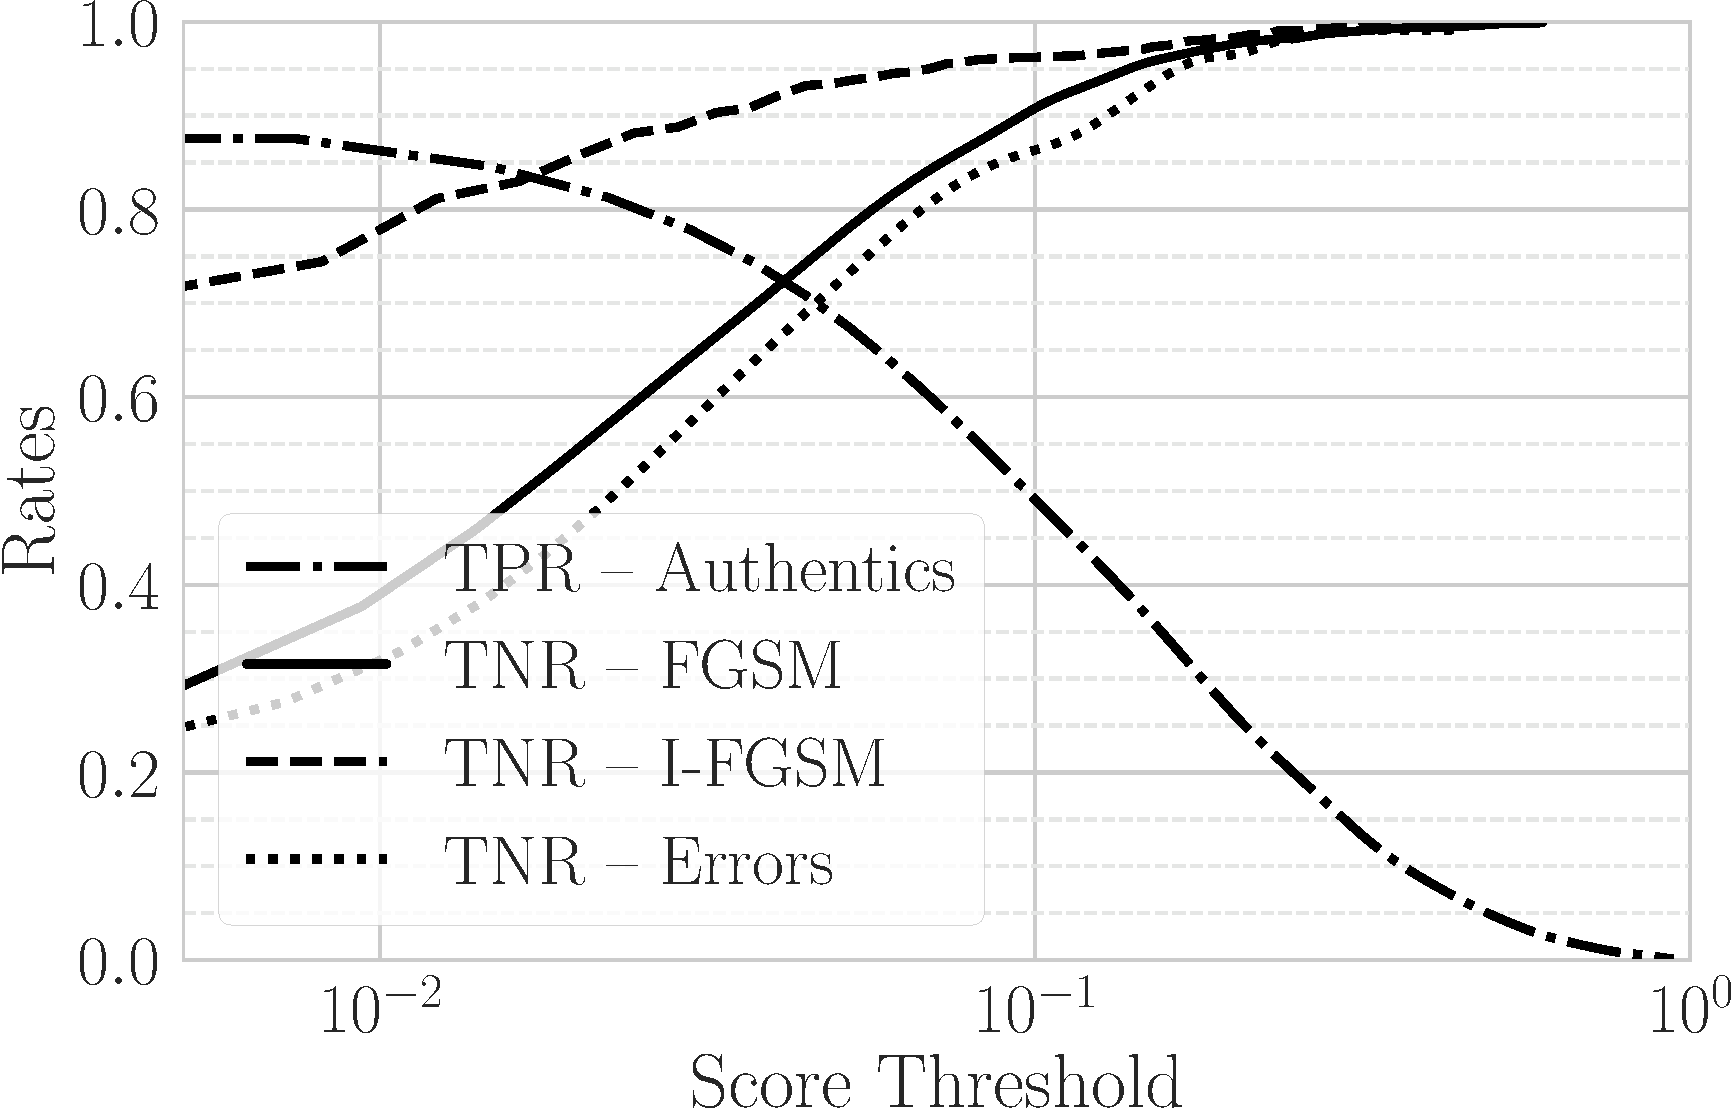
\includegraphics[width=\linewidth]{rates-mixed_6d-dwknn}%
\label{fig:adv:score-density-mixed_6e}%
\end{subfigure}%
%
\begin{subfigure}[t]{0.5\linewidth}%
\centering
\textbf{mixed\_7a}\\
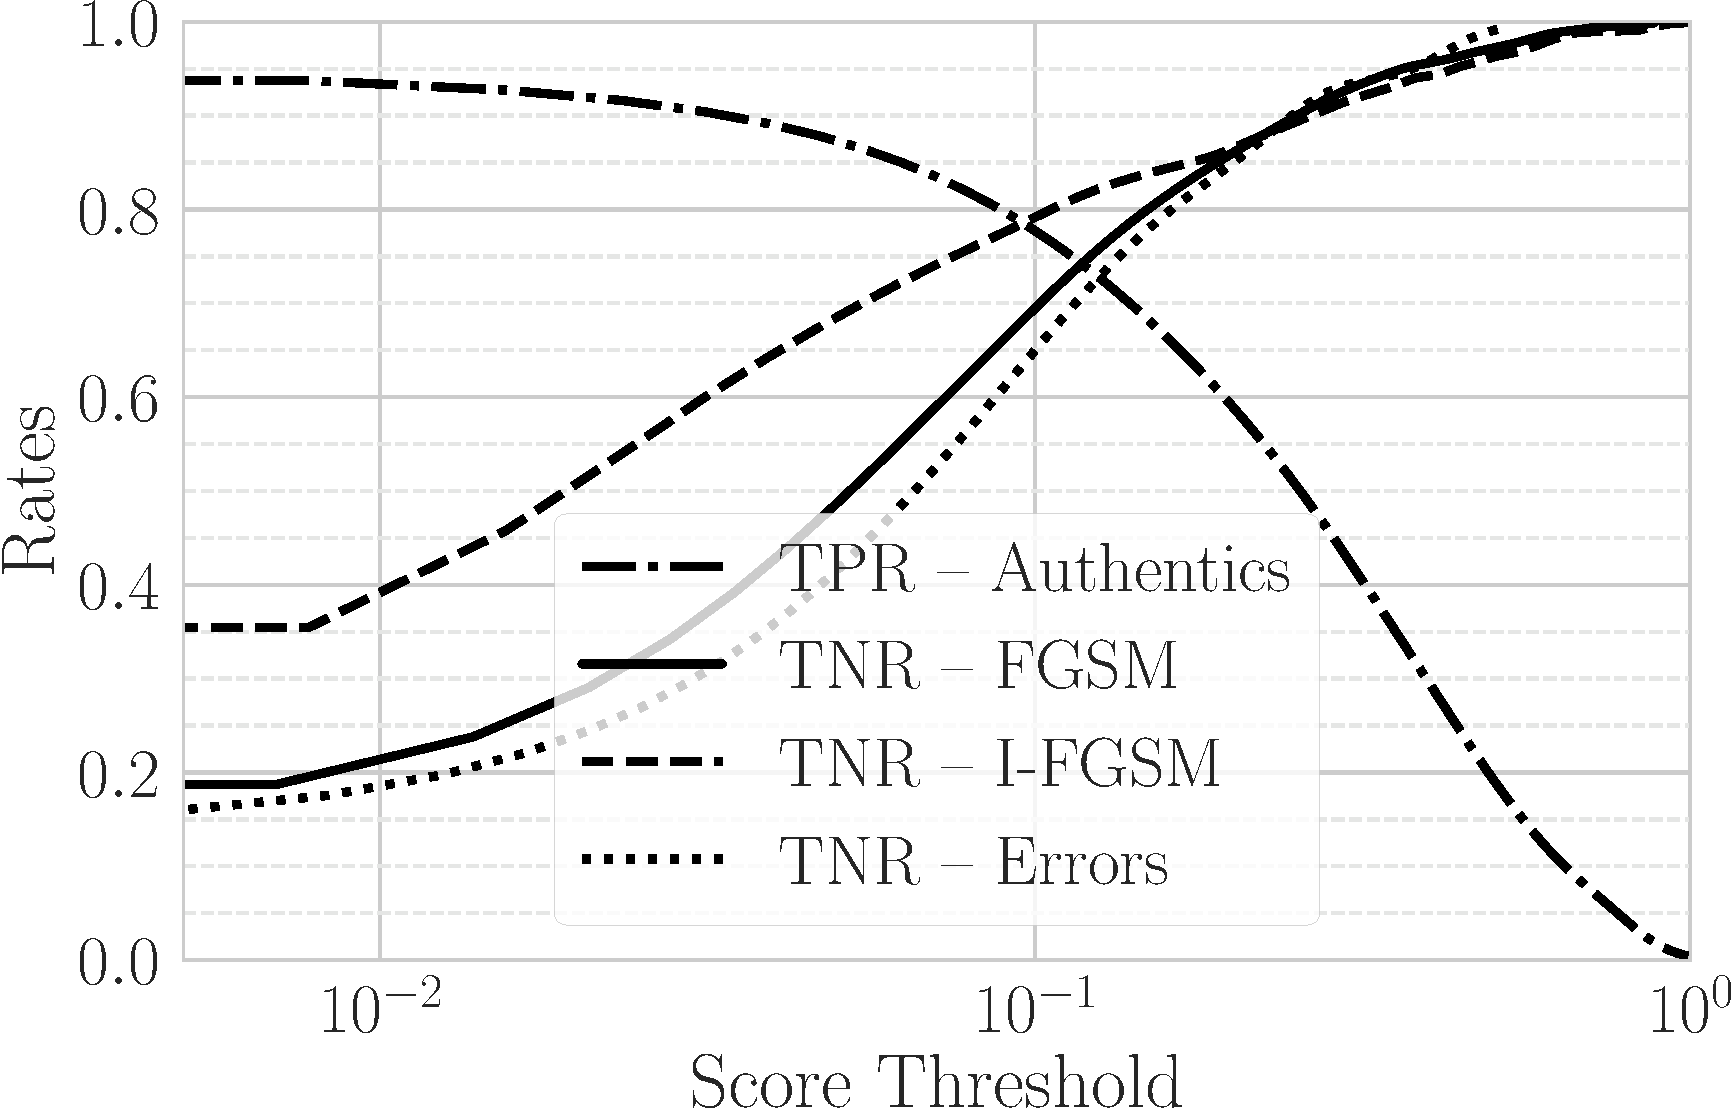
\includegraphics[width=\linewidth]{rates-mixed_7a-dwknn}%
\label{fig:adv:score-density-mixed_7a}%
\end{subfigure}%
%
\caption{True positive and false positive rates when varying the score threshold. The scores are computed using \textbf{\emph{mixed\_6d}} (on the left) and \textbf{\emph{mixed\_7a}} (on the right) of the InceptionV3 classifier.
DW-kNN scoring scheme was selected for both.}
\label{fig:adv:i3-distr}
\end{figure}

\begin{figure}
\centering
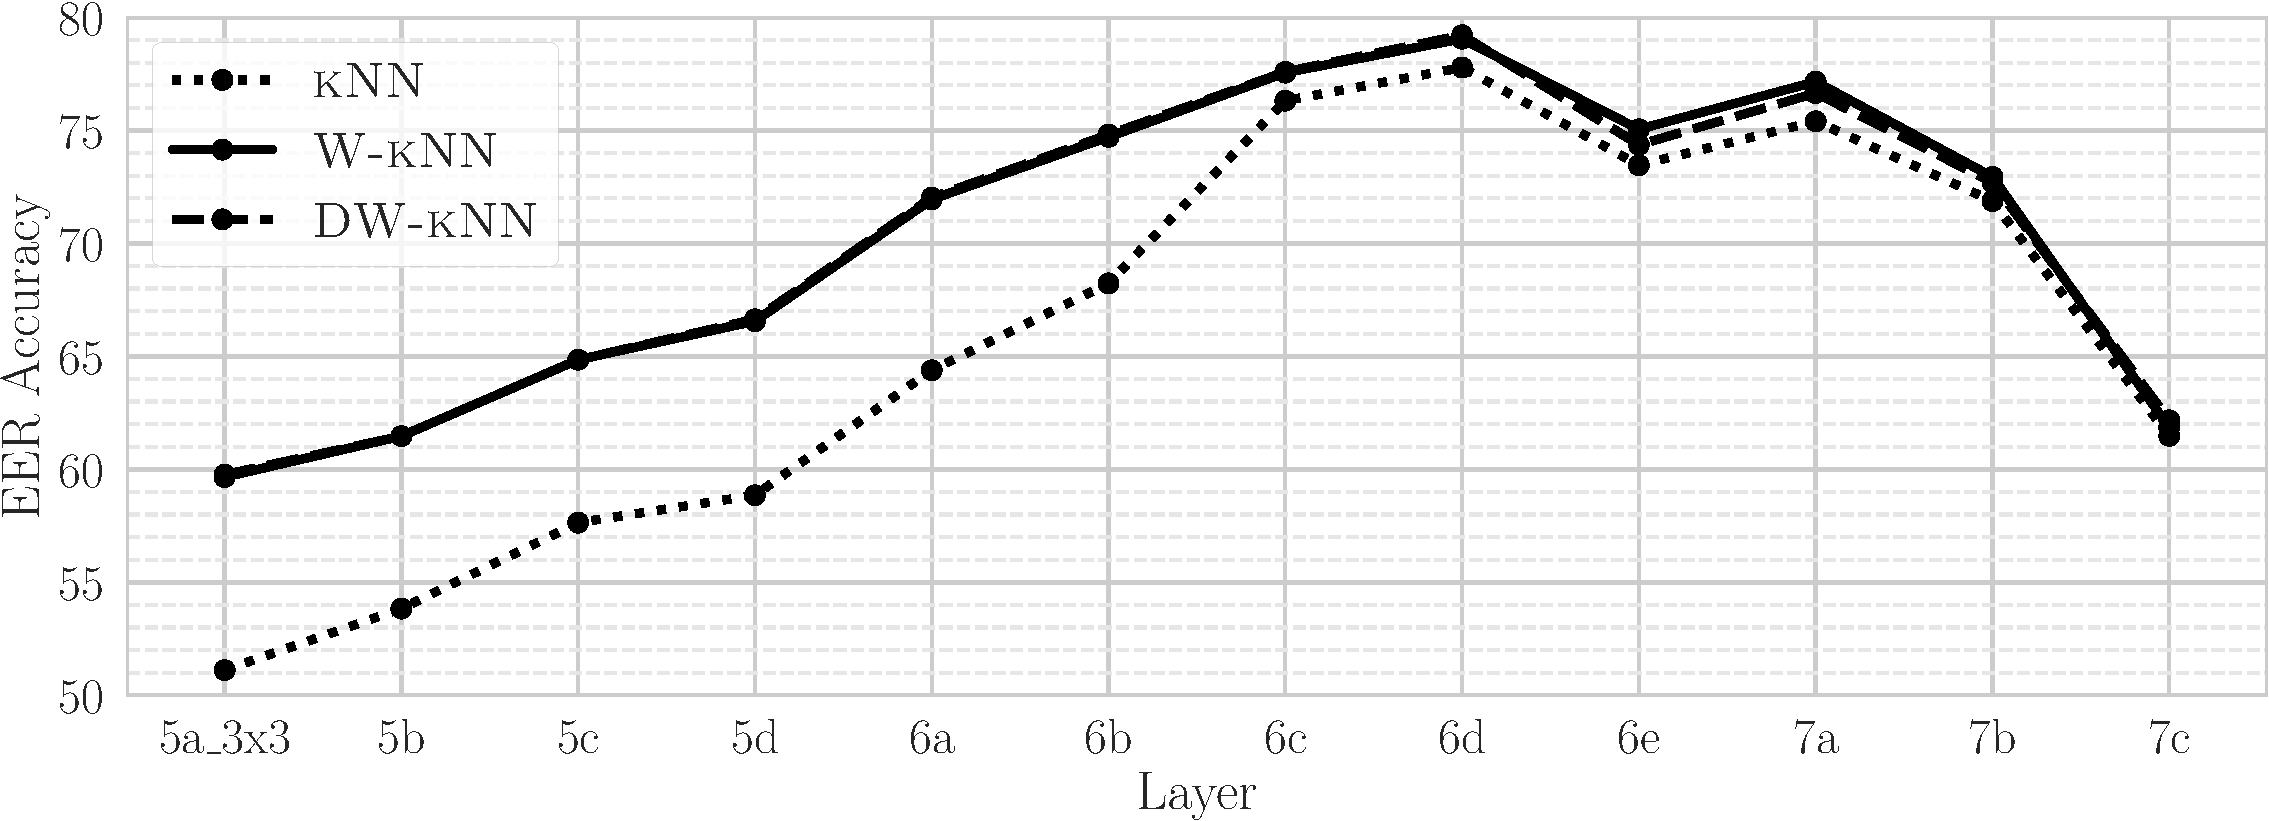
\includegraphics[width=\columnwidth]{incepv3-eer-acc}
\caption{The \acrlong{eer} accuracy obtained on the NIPS DEV set using different intermediate activations of the \emph{InceptionV3} as deep features.
Note that the effectiveness of the detection increases when using deeper representations and rapidly decreases when we reach the fooled layers at the end of the network.}
\label{fig:adv:i3-eer}
\end{figure}


\section{Summary}
\label{sec:adv:conclusions}

In this chapter, we presented an approach to detect adversarial examples crafted for fooling deep neural network classifiers.
The overall goal is filtering out malicious images.
To perform the detection, we relied on activations of neurons in hidden layers in order to detect adversarial examples.
In particular, we inspect the activations of intermediate layers for both adversarial and authentic inputs, and we defined an authenticity confidence score based on kNN similarity searching among the images used for training.
Experiments on the two most cited adversarial generation techniques (L-BFGS and \gls{fgsm}) on the very same neural network used in the original papers (i.e., OverFeat, InceptionV3) have been carried out.
In the experiments, we considered various kNN score functions and hidden layers.

%The results show that we were able to filter out roughly 85\% of adversarial images when looking to lower level activations (such as \emph{pool5}).
%Specifically, results shown that adversarials generated with L-BFGS are particularly difficult to detect.

When attacking the OverFeat model, the proposed approach allows to filter about 80\% of adversarial examples retaining more than 90\% of the correctly classified authentic images (see \ref{fig:adv:tptn-distribs}).
We also showed that the probability density function of our authenticity confidence obtained over adversarial examples significantly differs from the one obtained for authentic images.
%We showed that lower-level activations (such as \emph{pool5} with global average pooling) increase the detection performance with respect to the higher-level ones.
Moreover, some examples are suggesting that hard adversarial examples are the ones for which actual and target classes are similar or have similar visual patterns. %there are same visual patterns in both classes.

We also tested our method on the InceptionV3 \gls{cnn}, generating adversarial images from the NIPS 2017 Adversarial Attacks and Defenses Kaggle Competitions.
Using this dataset, we performed a thorough analysis of the detectability of adversarial examples when varying the internal layer extracted from the \gls{cnn}.
Best results were obtained using layer \emph{\textbf{mixed\_6d}} with an overall EER Accuracy of 80\%, confirming the effectiveness of our approach and its general applicability to deep neural network classifiers.
% TODO [MOVE] to conclusion chapter
%Future work may test the detection scheme under a more stringent threat model, in which the attacker is aware of the detection scheme used.
%The comparison of multiple layers for the detection performed in this study suggested that current adversarial crafting algorithms do not steer all the internal semantic representations inside the network, but focus on the last layers.
%Given these considerations, possible future work may also improve the presented detection scheme by relying on multiple intermediate layers, thus increasing the difficulty for a generation algorithm to craft adversarial images able to control multiple activations at once.